\documentclass[a4paper,10pt,twoside,openany]{book}

\usepackage[lang=hebrew]{maths}
\usepackage{polynom}
\usepackage{hebrewdoc}
\usepackage{stylish}
\usepackage{lipsum}
\let\bs\blacksquare

\renewcommand{\Mat}{\mathrm{M}}

\setlength{\parindent}{0pt}

%%%%%%%%%%%%
% Styling %
%%%%%%%%%%%%

\usepackage{enumitem}

%%%%%%%%%%%%%
% Counters  %
%%%%%%%%%%%%%

\setcounter{section}{1}     

%%%%%%%%%%%%%%%%%%%%%%%%%%%%%%%%%
% Boxes around matrix elements  %
%%%%%%%%%%%%%%%%%%%%%%%%%%%%%%%%%
\usepackage{tikz}
\usetikzlibrary{matrix,fit}
\pgfkeys{tikz/mymatrix/.style={matrix of math nodes,inner sep=0pt,row sep=0em,column sep=0em,nodes={inner sep=6pt}}}

\newcommand*\mymatrixbox[5][]{\node [fit= (m-#2-#3) (m-#4-#5)] [draw=blue,thick,dashed,rounded corners,inner sep=-2pt,#1] {};}            

\newcommand{\highlightcells}[2][]{%
  \foreach \r/\c in {#2} {%
    \mymatrixbox[#1]{\r}{\c}{\r}{\c}%
  }%
}
            
%BIBLIOGRAPHY
\usepackage[
backend=biber,
style=alphabetic,
]{biblatex}
\addbibresource{bibliography.bib} %Imports bibliography file

\title{
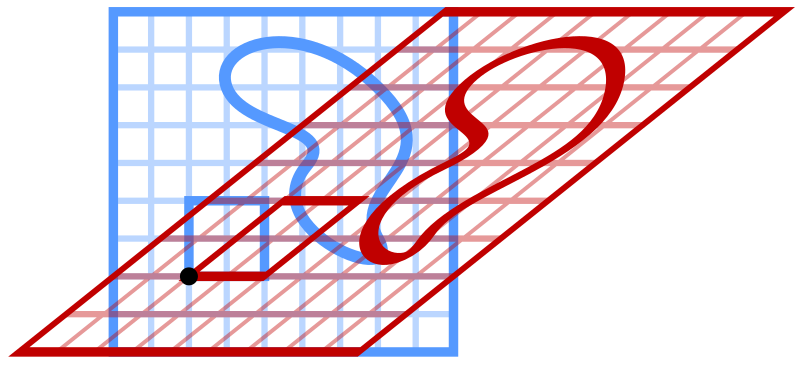
\includegraphics[width=6in]{images/front.png}\\
\vspace{30pt}
\Huge
אלגברה ב' (01040168)
\\
אביב 2026
\\
רשימות תרגולים
\vspace{30pt}
\\
\huge
אלן סורני
\vspace{30pt}
\\
\Large
הרשימות עודכנו לאחרונה בתאריך ה־%
\today
}
\date{}

\begin{document}
\frontmatter
\maketitle
\tableofcontents

\mainmatter

\section*{סימונים}

\begin{itemize}
\item[-]
$\brs{n} = \set{1, \ldots, n}$.
\item[-]
$\sum_{i \in \brs{n}} a_i = \sum_{i=1}^n a_i = a_1 + a_2 + \ldots + a_n$
\item[-] $\Mat_{m \times n}\prs{\mbb{F}}$ הוא מרחב המטריצות עם
$m$
שורות ו־%
$n$
עמודות, עם מקדמים בשדה
$\mbb{F}$.
\item[-]
$\mbb{F}^n = \Mat_{n \times 1}\prs{\mbb{F}}$
\item[-]
$\Mat_{n}\prs{\mbb{F}} = \Mat_{n \times n}\prs{\mbb{F}}$
\item[-]
$\hom_{\mbb{F}}\prs{V,W}$
הוא מרחב ההעתקות הלינאריות
$V \to W$
כאשר
$V,W$
מרחבים וקטוריים מעל
$\mbb{F}$.
\item[-]
$\End_{\mbb{F}}\prs{V} = \hom_{\mbb{F}}\prs{V,V}$
\item[-]
אותיות בפונט
\textenglish{mathcal}
עבור בסיסים -
$\mcal{B}, \mcal{C}, \mcal{D}$
וכו'
\end{itemize}

\part{חלק ראשון - מרחבים שמורים}

\chapter{חזרה על מטריצות מייצגות}

\section{הגדרות ותכונות בסיסיות}

\begin{definition}[וקטור קואורדינטות]
יהי
$V$
מרחב וקטורי סוף־מימדי מעל שדה
$\mbb{F}$,
יהי
$\mcal{B} = \prs{v_1, \ldots, v_n}$
בסיס של
$V$
ויהי
$v \in V$.
\emph{וקטור הקואורדינטות של
$v$
לפי הבסיס
$B$}
הוא הוקטור
$\brs{v}_\mcal{B} = \pmat{\alpha_1 \\ \vdots \\ \alpha_n}$
כאשר
$\alpha_1, \ldots, \alpha_n \in \mbb{F}$
היחידים עבורם
\[\text{.}v = \sum_{i \in [n]} \alpha_i v_i \coloneqq \alpha_1 v_1 + \ldots + \alpha_n v_n\]
\end{definition}

\begin{remark}
ההעתקה
\begin{align*}
\rho_\mcal{B} \colon V &\to \mbb{F}^n \\
v &\mapsto \brs{v}_\mcal{B}
\end{align*}
היא איזומורפיזם לינארי.
\end{remark}

\begin{definition}[מטריצה מייצגת]
יהיו
$V,W$
מרחבים וקטורים סוף־מימדיים מעל אותו שדה
$\mbb{F}$
עם בסיסים
$\mcal{B}, \mcal{C}$
בהתאמה, ונסמן
\[\text{.} \mcal{B} = \prs{v_1, \ldots, v_n}\]
נסמן גם
$n \coloneqq \dim\prs{V}$
ו־%
$m \coloneqq \dim\prs{W}$.
עבור
$T \in \Hom_{\mbb{F}}\prs{V,W}$
נגדיר
\[\text{.} \brs{T}^\mcal{B}_\mcal{C} = \pmat{\vert & & \vert \\ \brs{T\prs{v_1}}_\mcal{C} & \cdots & \brs{T\prs{v_n}}_\mcal{C} \\ \vert & & \vert} \in \Mat_{m \times n}\prs{\mbb{F}}\]
\end{definition}

\begin{theorem}[כפל מטריצות]
תהי
$A \in \Mat_{m \times n}\prs{\mbb{F}}$
ויהי
$\mcal{E} = \prs{e_1, \ldots, e_m}$
הבסיס הסטנדרטי של
$\mbb{F}^n$.
אז:
\begin{enumerate}[label = (\roman*)]
\item
לכל
$i \in [m]$
מתקיים כי
$A e_i$
העמודה ה־%
$i$
של
$A$.
\item
לכל
$B = \pmat{\vert & & \vert \\ b_1 & \cdots & b_\ell \\ \vert & & \vert} \in \Mat_{n \times \ell}\prs{\mbb{F}}$
מתקיים
$AB = \pmat{\vert & & \vert \\ A b_1 & \cdots & A b_\ell \\ \vert & & \vert}$.
\end{enumerate}
\end{theorem}

\begin{exercisechap}
הראו שניתן לשחזר את ההגדרה של כפל מטריצות משתי התכונות במשפט.
\end{exercisechap}

\begin{remark}
ההעתקה
\begin{align*}
\eta^\mcal{B}_\mcal{C} \colon \Hom_{\mbb{F}}\prs{V,B} &\to \Mat_{m \times n}\prs{\mbb{F}} \\
T &\mapsto \brs{T}^\mcal{B}_\mcal{C}
\end{align*}
היא איזומורפיזם לינארי.
\end{remark}

\begin{proposition}
תהי
$T \in \Hom_{\mbb{F}}\prs{V,W}$
ויהיו
$\mcal{B} = \prs{v_1, \ldots, v_n}$
בסיס של
$V$
ו־%
$\mcal{C}$
בסיס של
$W$.
אז
\[\brs{T}^\mcal{B}_\mcal{C} \brs{v}_\mcal{B} = \brs{T\prs{v}}_\mcal{C}\]
לכל
$v \in V$.
\end{proposition}

\begin{notation}
אם
$\mcal{B}$
בסיס של מרחב וקטורי סוף־מימדי
$V$
ואם
$T \in \End\prs{V}$,
נסמן
$\brs{T}_\mcal{B} \coloneqq \brs{T}^\mcal{B}_\mcal{B}$
ונקרא למטריצה זאת
\emph{המטריצה המייצגת של
$T$
לפי הבסיס
$\mcal{B}$}.
\end{notation}

\begin{notation}
יהי
$V$
מרחב וקטורי סוף־מימדי עם בסיסים
$\mcal{B},\mcal{C}$.
נסמן
$M^\mcal{B}_\mcal{C} \coloneqq \brs{\id_V}^\mcal{B}_\mcal{C}$.
\end{notation}

\begin{notation}
אם
$A \in \Mat_{n\times n}\prs{\mbb{F}}$,
נסמן
\begin{align*}
T_A \colon \mbb{F}^n &\to \mbb{F}^n \\
\text{.} \hphantom{lalala} v &\mapsto Av
\end{align*}
\end{notation}

\section{תרגילים}

\begin{exercisechap}
תהי
$A \in \Mat_n\prs{\FF}$
ויהי
$\mcal{E} = \prs{e_1, \ldots, e_n}$
הבסיס הסטנדרטי של
$\FF^n$.
הראו כי
$\brs{T_A}_{\mcal{E}} = A$.
\end{exercisechap}

\begin{solution}
לפי הגדרת מטריצה מייצגת, העמודה ה־%
$i$
של
$\brs{T_A}_{\mcal{E}}$
היא
$T_A \prs{e_i} = A e_i$.
לפי הגדרת כפל מטריצות, וכפי שראינו באלגברה א', זאת בדיוק העמודה ה־%
$i$
של
$A$.
\end{solution}

\begin{exercisechap}\label{ex:p(x+1)}
יהי
$V = \mbb{R}_3\brs{x}$
מרחב הפולינום הממשיים ממעלה לכל היותר
$3$,
תהי
\begin{align*}
T \colon \mbb{R}_3\brs{x} &\to \mbb{R}_3\brs{x} \\
p\prs{x} &\mapsto p\prs{x+1}
\end{align*}
ויהי
$\mcal{B} = \prs{1,x,x^2,x^3}$
בסיס של
$V$.
כיתבו את
$\brs{T}_\mcal{B}$.
\end{exercisechap}

\begin{solution}
לפי הגדרת המטריצה המייצגת,
עמודות
$\brs{T}_\mcal{B}$
הן
$\brs{T\prs{x^i}}_B$
עבור
$i \in \set{0,1,2,3}$.
מתקיים
\begin{align*}
T\prs{1} &= 1 \\
T\prs{x} &= x+1 = 1 + x \\
T\prs{x^2} &= \prs{x+1}^2 = 1 + 2x + x^2 \\
T\prs{x^3} &= \prs{x+1}^3 = 1 + 3x + 3x^2 + x^3
\end{align*}
ולכן
\begin{align*}
\brs{T\prs{1}}_\mcal{B} &= e_1 \\
\brs{T\prs{x}}_\mcal{B} &= e_1 + e_2 \\
\brs{T\prs{x^2}}_\mcal{B} &= e_1 + 2 e_2 + e_3 \\
\brs{T\prs{x^3}}_\mcal{B} &= e_1 + 3 e_2 + 3 e_3 + e_4
\end{align*}
ואז
\begin{align*}
\text{.} \brs{T}_\mcal{B} &= \pmat{1 & 1 & 1 & 1 \\ 0 & 1 & 2 & 3 \\ 0 & 0 & 1 & 3 \\ 0 & 0 & 0 & 1}
\end{align*}
\end{solution}

\begin{exercisechap}
יהי
$V = \Mat_{2 \times 2}\prs{\mbb{C}}$,
תהי
\begin{align*}
T \colon V &\to V \\
A &\mapsto \frac{1}{2} \prs{A - A^t}
\end{align*}
ויהי
\[\mcal{E} = \prs{E_{1,1}, E_{1,2}, E_{2,1}, E_{2,2}} \coloneqq \pmat{\pmat{1 & 0 \\ 0 & 0}, \pmat{0 & 1 \\ 0 & 0}, \pmat{0 & 0 \\ 1 & 0}, \pmat{0 & 0 \\ 0 & 1}}\]
\emph{הבסיס הסטנדרטי של
$V$}.
כיתבו את
$\brs{T}_\mcal{E}$.
\end{exercisechap}

\begin{solution}
כמו מקודם, נחשב את
$\brs{T\prs{E_{i,j}}}_\mcal{E}$
כיוון שאלו עמודות
$\brs{T}_\mcal{E}$.
מתקיים
\begin{align*}
T\prs{E_{1,1}} &= \frac{1}{2} \prs{E_{1,1} - E_{1,1}} = 0 \\
T\prs{E_{1,2}} &= \frac{1}{2} \prs{\pmat{0 & 1 \\ 0 & 0} - \pmat{0 & 0 \\ 1 & 0}} = \frac{1}{2} E_{1,2} - \frac{1}{2} E_{2,1} \\
T\prs{E_{2,1}} &= \frac{1}{2} \prs{E_{2,1} - E_{1,2}} = \frac{1}{2} E_{2,1} - \frac{1}{2} E_{1,2} \\
\text{,} T\prs{E_{2,2}} &= \frac{1}{2} \prs{E_{2,2} - E_{2,2}} = 0 \\
\end{align*}
לכן
\begin{align*}
\brs{T\prs{E_{1,1}}}_\mcal{E} &= 0 \\
\brs{T\prs{E_{1,2}}}_\mcal{E} &= \frac{1}{2} e_2 - \frac{1}{2} e_3 \\
\brs{T\prs{E_{2,1}}}_\mcal{E} &= -\frac{1}{2} e_2 + \frac{1}{2} e_3 \\
\brs{T\prs{E_{2,2}}}_\mcal{E} &= 0
\end{align*}
ואז
\begin{align*}
\text{,} \brs{T}_\mcal{E} &= \pmat{0 & 0 & 0 & 0 \\ 0 & \frac{1}{2} & -\frac{1}{2} & 0 \\ 0 & -\frac{1}{2} & \frac{1}{2} & 0 \\ 0 & 0 & 0 & 0}
\end{align*}
כנדרש.
\end{solution}

\begin{exercisechap}
תהיינה
$A,B \in \Mat_{m \times n}\prs{\mbb{F}}$
ונניח כי לכל
$v \in \mbb{F}^n$
מתקיים
$Av = Bv$.
אז
$A = B$.
\end{exercisechap}

\begin{solution}
מהנתון, מתקיים
$\prs{A - B}v = 0$
לכל
$v \in \mbb{F}^n$.
בפרט העמודה ה־%
$i$
של
$A-B$,
שהינה
$\prs{A - B}e_i$,
שווה ל־%
$0$.
לכן
$A - B = 0$.
\end{solution}

\begin{proposition}
יהיו
$U,V,W$
מרחבים וקטוריים סוף־מימדיים מעל אותו שדה
$\mbb{F}$
עם בסיסים
$\mcal{B},\mcal{C},\mcal{D}$
בהתאמה,
ותהיינה
\begin{align*}
S \in \Hom_{\mbb{F}}\prs{U,V} \\
\text{.} T \in \Hom_{\mbb{F}}\prs{V,W}
\end{align*}
אז
\[\text{.} \brs{T \circ S}^\mcal{B}_\mcal{D} = \brs{T}^\mcal{C}_\mcal{D} \brs{S}^\mcal{B}_\mcal{C}\]
\end{proposition}

\begin{exercisechap}
תהיינה
\begin{align*}
A &\coloneqq \pmat{0 & 1 \\ -1 & 0} \in \Mat_2\prs{\RR} \\
\text{.} B &\coloneqq \pmat{1 & 0 \\ 0 & -1} \in \Mat_2\prs{\RR}
\end{align*}
מבלי לכפול מטריצות, מיצאו העתקה לינארית
$T \in \End_{\RR}\prs{\RR^2}$
עבורה
$\brs{T}_{\mcal{E}} = AB$.
\end{exercisechap}

\begin{solution}
יהי
$\mcal{E}$
הבסיס הסטנדרטי של
$\RR^2$.
לפי הטענה האחרונה, מתקיים
\begin{align*}
\brs{T_A \circ T_B}_{\mcal{E}} = \brs{T_A}_{\mcal{E}} \brs{T_B}_{\mcal{E}}
\end{align*}
אך כפי שראינו מתקיים
\begin{align*}
\brs{T_A}_{\mcal{E}} = A \\ \brs{T_B}_{\mcal{E}} = B
\end{align*}
ולכן בסך הכל
\begin{align*}
\brs{T_A \circ T_B} = AB
\end{align*}
ונבחר את האופרטור
$T = T_A \circ T_B$
שיקיים
$\brs{T}_{\mcal{E}} = AB$
כנדרש.

נחשב אותו מפורשות. מתקיים
\begin{align*}
T_A \pmat{x \\ y} &= \pmat{0 & 1 \\ -1 & 0} \pmat{x \\ y}
\\&=
\pmat{0 & 1 \\ -1 & 0} \prs{x e_1 + y e_2}
\\&=
x \pmat{0 & 1 \\ -1 & 0} e_1 + y \pmat{0 & 1 \\ -1 & 0} e_2
\\&=
x \pmat{0 \\ -1} + y \pmat{1 \\ 0}
\\&= 
\pmat{y \\ -x}
\end{align*}
וכן
\begin{align*}
T_B\pmat{x \\ y} &= \pmat{1 & 0 \\ 0 & -1} \pmat{x \\ y}
\\&=
x \pmat{1 & 0 \\ 0 & -1} e_1 + y \pmat{1 & 0 \\ 0 & -1} e_2
\\&=
x \pmat{1 \\ 0} + y \pmat{0 \\ -1}
\\&=
\pmat{x \\ -y}
\end{align*}
ולכן
\begin{align*}
T\pmat{x \\ y} &= \prs{T_A \circ T_B} \pmat{x \\ y}
\\&=
T_A\prs{T_B\pmat{x \\ y}}
\\&=
T_A\pmat{x \\ -y}
\\&=
\pmat{-y \\ -x}
\end{align*}
כנדרש.
\end{solution}

\chapter{הדטרמיננטה}

\section{הגדרות ותכונות בסיסיות}

\begin{definition}[דטרמיננטה]
תהי
$A \in \Mat_{n \times n}\prs{\mbb{F}}$
מטריצה עם מקדמים בשדה
$\mbb{F}$.
נגדיר את
\emph{הדטרמיננטה}
$\det\prs{A}$
של
$A$
באופן הרקורסיבי הבא.

תהי
$A_{\prs{i,j}}$
המטריצה המתקבלת מ־%
$A$
על ידי הסרת השורה ה־%
$i$
והעמודה ה־%
$j$.
המספר
$\det\prs{A_{\prs{i,j}}}$
נקרא
\emph{המינור}
ה־$\prs{i,j}$ של
$A$
והדטרמיננטה של
$A$
שווה
\begin{align*}
\det\prs{A} &= \sum_{i \in \brs{n}} \prs{-1}^{i+j} a_{i,j} \det\prs{A_{\prs{i,j}}}
\end{align*}
עבור כל
$j \in \brs{n}$
קבוע, ושווה
\begin{align*}
\det\prs{A} &= \sum_{j \in \brs{n}} \prs{-1}^{i+j} a_{i,j} \det\prs{A_{\prs{i,j}}}
\end{align*}
עבור כל
$i \in \brs{n}$
קבוע.
\end{definition}

\begin{theorem}
תהיינה
$A, B, C \in \Mat_{n \times n}\prs{\mbb{F}}$
ונניח כי
$C$
הפיכה.
מתקיימות התכונות הבאות.
\begin{enumerate}
\item $\det\prs{AB} = \det\prs{A} \cdot \det\prs{B}$
\item $\det\prs{C^{-1}} = \prs{\det\prs{C}}^{-1}$
\end{enumerate}
\end{theorem}

\begin{theorem}
\begin{enumerate}
\item החלפת שתי שורות או עמודות במטריצה כופלת את הדטרמיננטה ב־%
$\prs{-1}$.
\item כפל שורה או עמודה במטריצה בסקלר
$\alpha$
כופל את הדטרמיננטה ב־%
$\alpha$.
\item הוספת כפולה שורה או עמודה לשורה או עמודה במטריצה אינה משנה את הדטרמיננטה.
\end{enumerate}
\end{theorem}

\section{תרגילים}

\begin{exercisechap}
חשבו את הדטרמיננטות של המטריצות הבאות.

\begin{enumerate}
\item \[\pmat{1 & 2 & 3 \\ 4 & 5 & 6 \\ 7 & 8 & 9} \in \Mat_{3}\prs{\mbb{R}}\]
\item \[\pmat{0 & 0 & 0 & 1 \\ 0 & 0 & 1 & 0 \\ 0 & 1 & 0 & 0 \\ 1 & 0 & 0 & 0} \in \Mat_{4}\prs{\mbb{R}}\]
\item \[\pmat{1 & 0 & 0 \\ 0 & 1 & 0 \\ 1 & 1 & 1} \in \Mat_{3}\prs{\mbb{R}}\]
\item \[\pmat{1 & 0 & 1 \\ 0 & 1 & 0 \\ 1 & 1 & 1} \in \Mat_{3}\prs{\mbb{R}}\]
\end{enumerate}
\end{exercisechap}

\begin{solution}
\begin{enumerate}
\item
נחשב לפי השורה הראשונה.
\begin{align*}
\det \pmat{1 & 2 & 3 \\ 4 & 5 & 6 \\ 7 & 8 & 9} &= 1 \cdot \det\pmat{5 & 6 \\ 8 & 9} - 2 \cdot \det \pmat{4 & 6 \\ 7 & 9} + 3 \cdot \det \pmat{4 & 5 \\ 7 & 8}
\\&=
1 \cdot \prs{5 \cdot 9 - 6 \cdot 8} - 2 \cdot \prs{4 \cdot 9 - 6 \cdot 7} + 3 \cdot \prs{4 \cdot 8 - 5 \cdot 7}
\\&=
1 \cdot \prs{-3} -2 \cdot \prs{-6} + 3 \cdot \prs{-3}
\\&=
-3 + 12 - 9
\\&= 0
\end{align*}
\item החלפת שורות כופלת את הדטרמיננטה ב־%
$\prs{-1}$.
כיוון שניתן לקבל את המטריצה ממטריצת היחידה על ידי החלפת השורות
$1,4$
והשורות
$2,3$,
נקבל כי הדטרמיננטה שווה לזאת של היחידה. לכן
\[\text{.} \det \pmat{0 & 0 & 0 & 1 \\ 0 & 0 & 1 & 0 \\ 0 & 1 & 0 & 0 \\ 1 & 0 & 0 & 0} = 1\]
\item
הוספת כפולה של השורות הראשונה והשנייה ב־%
$\prs{-1}$
לשורה השלישית לא משנה את הדרמיננטה. לכן הדטמיננטה של המטריצה שווה לזאת של היחידה, ולכן
\[\text{.} \det \pmat{1 & 0 & 0 \\ 0 & 1 & 0 \\ 1 & 1 & 1} = 1\]
\item
הוספת כפולה של השורות הראשונה והשנייה ב־%
$\prs{-1}$
לשורה השלישית לא משנה את הדרמיננטה. לכן הדטמיננטה של המטריצה שווה לזאת של
\begin{align*}
\text{.} \pmat{1 & 0 & 1 \\ 0 & 1 & 0 \\ 0 & 0 & 0}
\end{align*}
כיוון שהשורה השלישית היא שורת אפסים, אם נפתח את הדטרמיננטה לפיה נקבל שהדטרמיננטה שווה
$0$.
זה נכון באופן כללי יותר אם השורות תלויות לינארית, כי נוכל לקבל שורת אפסים מצירוף לינארי של השורות.
\end{enumerate}
\end{solution}

\begin{exercisechap}
תהי
$T \in \End_{\mbb{F}}\prs{V}$
העתקה לינארית ויהי
$\mcal{B}$
בסיס של
$V$.
הראו כי ניתן להגדיר
$\det\prs{T} = \det\prs{\brs{T}_\mcal{B}}$.
כלומר, הראו שאם
$\mcal{C}$
בסיס נוסף של
$V$
מתקיים
$\det\prs{\brs{T}_\mcal{B}} = \det\prs{\brs{T}_\mcal{C}}$.
\end{exercisechap}

\begin{solution}
מתקיים
\begin{align*}
\brs{T}_\mcal{B} = \prs{M^\mcal{B}_\mcal{C}}^{-1} \brs{T}_\mcal{C} M^\mcal{B}_\mcal{C}
\end{align*}
ולכן
\begin{align*}
\text{.} \det\prs{\brs{T}_\mcal{B}} &= \det\prs{\prs{M^\mcal{B}_\mcal{C}}^{-1}} \det\prs{\brs{T}_\mcal{C}} \det\prs{M^\mcal{B}_\mcal{C}}
\end{align*}
כיוון ש־%
$\det\prs{A^{-1}} = \frac{1}{\det\prs{A}}$
 לכל מטריצה
 $A$,
 מתקיים
 $\det\prs{\prs{M^\mcal{B}_\mcal{C}}^{-1}} = \frac{1}{\det\prs{M^\mcal{B}_\mcal{C}}}$.
 לכן, נקבל בסה"כ כי
 \[\text{,} \det\prs{\brs{T}_\mcal{B}} = \det\prs{\brs{T}_\mcal{C}}\]
 כנדרש.
\end{solution}

\section{הדטרמיננטה לפי תמורות}

\begin{definition}[תמורות על $n$ איברים]
העתקה
\[\sigma \colon [n] \to [n]\]
נקראת
\emph{תמורה על $[n]$}
אם היא חד־חד־ערכית ועל.

אוסף כל התמורות על
$[n]$
מסומן
$S_n$,
ונסמן
$\sigma \tau$
עבור ההרכבה
$\sigma \circ \tau$
של איברים בו.
\end{definition}

\begin{definition}[חילוף]
תמורה
$\sigma \in S_n$
נקראת
\emph{חילוף}
אם קיימים
$i,j \in [n]$
שונים עבורם
\begin{align*}
\sigma\prs{i} &= j \\
\sigma\prs{j} &= i \\
\text{.} \forall k \in [n] \setminus \set{i,j} : \sigma\prs{k} &= k
\end{align*}
\end{definition}

\begin{notation}
נסמן תמורה
$\sigma \in S_n$
בתור
$\sigma = \prs{\sigma\prs{1}, \ldots, \sigma\prs{n}}$,
וחילוף
$\tau$
בין איברים
$n,m$
בתור
$\prs{n;m}$.
\end{notation}

\begin{definition}[סימן של תמורה]
ראיתן בהרצאה כי כל תמורה
$\sigma$
ניתן לכתיבה כהרכבה של חילופים
$\tau_1, \ldots, \tau_m$,
וכי אם היא הרכבה גם של חילופים
$\tau_1', \ldots, \tau_k'$
אז
$\prs{-1}^m = \prs{-1}^k$.

לכן, ניתן להגדיר את
\emph{הסימן של תמורה
$\sigma$}
בתור
$\prs{-1}^k$
כאשר
$k$
מספר החילופים בהצגת
$\sigma$
כהרכבת חילופים.
נסמנו
$\sgn\prs{\sigma}$.
\end{definition}

\begin{exercisechap}
חשבו את הסימן של התמורה
\[\text{.} \sigma \coloneqq \prs{n, 1, 2, \ldots, \prs{n-1}} \in S_n\]
\end{exercisechap}

\begin{solution}
הסימן של
$\sigma$
הוא
$\prs{-1}$
בחזקת מספר החילופים בהצגת
$\sigma$
כהרכבת חילופים.

אם נמצא חילופים
$\tau_1, \ldots, \tau_k$
עבורם
\[\tau_k \circ \ldots \circ \tau_1 \sigma = \id_{[n]}\]
נקבל כי
\[\sigma^{-1} = \tau_k \circ \ldots \circ \tau_1\]
ולכן
\begin{align*}
\sigma &= \prs{\tau_k \circ \ldots \circ \tau_1}^{-1}
\\&= \tau_1^{-1} \circ \ldots \circ \tau_k^{-1}
\\&= \tau_1 \circ \ldots \circ \tau_k
\end{align*}
ואז
$\sgn\prs{\sigma} = \prs{-1}^k$.

נבצע חילופים כאלו כאשר נדאג, משמאל לימין, שהערכים של התמורה החדשה נשלחים לעצמם.
מתקיים
\begin{align*}
\prs{1;n} \sigma &= \prs{1, n, 2, 3, \ldots, \prs{n-1}} \\
\prs{2;n} \prs{1;n} \sigma &= \prs{1, 2, n, 3, \ldots, \prs{n-1}} \\
\vdots \\
\prs{n-1;n} \circ \ldots \circ \prs{1;n} \sigma &= \id_{[n]}
\end{align*}
ולכן
\[\sigma = \prs{1;n} \prs{2;n} \circ \ldots \circ \prs{n-1;n}\]
ואז
\[\text{,} \sgn\prs{\sigma} = \prs{-1}^{n-1}\]
כנדרש.
\end{solution}

בהרצאות הקרובות, תיראו כי ניתן לחשב דטרמיננטה בעזרת תמורות באופן הבא.

\begin{proposition}
תהי
$A = \prs{a_{i,j}}_{i,j \in \brs{n}} \in \Mat_n\prs{\mbb{F}}$.
מתקיים
\[\text{.} \det\prs{A} = \sum_{\sigma \in S_n} \sgn{\sigma} \prod_{i \in \brs{n}} a_{i,\sigma\prs{i}}\]
\end{proposition}

\begin{remark}
כל תמורה ב־%
$S_n$
מתאימה לבחירה של סדר על איברי
$[n]$,
ולכן בסכום מתאימה לבחירה של מקדם מכל שורה, כך שמכל עמודה נבחר רק מקדם אחד.
נסכום את מכפלות המקדמים מהבחירות השונות, כאשר חלק מהמכפלות האלו יסכמו בסימן שלילי, לפי סימן התמורות המתאימות להן.

למשל, אם
\[A = \pmat{1 & 2 \\ 3 & 4}\]
נסתכל על התמורות ב־%
$S_2$:
\[\sigma_1 \coloneqq \prs{1, 2}, \sigma_2 \coloneqq \prs{2, 1}\]
ומתקיים
\begin{align*}
\sgn\prs{\sigma_1} &= \sgn\prs{\prs{1, 2}} = \sgn\prs{\id_{[2]}} = \prs{-1}^0 = 1 \\
\text{.} \sgn\prs{\sigma_2} &= \sgn\prs{\prs{2, 1}} = \prs{-1}^1 = -1
\end{align*}
הדטרמיננטה, לפי ההגדרה, היא
\begin{align*}
\prs{\sgn\prs{\sigma_1} \prod_{i \in [2]} a_{i, \sigma_1\prs{i}}} + \prs{\sgn\prs{\sigma_2} \prod_{i \in [2]} a_{i, \sigma_2\prs{i}} }
&=
a_{1, \sigma_1\prs{1}} a_{2, \sigma_1\prs{2}} - a_{1, \sigma_2(1)} a_{2, \sigma_2(2)}
\\&=
a_{1,1} a_{2,2} - a_{1,2} a_{2,1}
\\&= 1 \cdot 4 - 2 \cdot 3
\\&= -2
\end{align*}
כאשר הגורם בסכום הנ"ל שמתאים לתמורה
$\prs{1 2}$
הוא המכפלה של המקדם ה־%
$1$
בשורה הראשונה והמקדם ה־%
$2$
בשורה השנייה, והגורם המתאים לתמורה
$\prs{2 1}$
הוא (מינוס) המכפלה של המקדם ה־%
$2$
בשורה ה־%
$1$
והמקדם ה־%
$1$
בשורה השנייה, כפול סימן התמורה שהוא
$-1$.

\end{remark}

\begin{exercisechap}
חשבו את הדטרמיננטה של המטריצה הבאה לפי תמורות.

\begin{align*}
\text{.} A = \pmat{1 & 2 & 3 \\ 4 & 5 & 6 \\ 7 & 8 & 9}
\end{align*}
\end{exercisechap}

\begin{solution}
נרשום את כל איברי
$S_3$.
הם
\begin{align*}
\id_{S_3} &= \prs{1, 2, 3}, \\
&\hphantom{=} \prs{1, 3, 2}, \\
&\hphantom{=} \prs{2, 1, 3}, \\
&\hphantom{=} \prs{2, 3, 1}, \\
&\hphantom{=} \prs{3, 1, 2}, \\
\text{.} \hphantom{\id_{S_3}} &\hphantom{=} \prs{3, 2, 1}
\end{align*}
עבור כל אחד מהאיברים, נפעיל חילופים משמאל כדי להביא אותו ליחידה, ומספר החילופים יהיה החזקה של $\prs{-1}$ בסימן של התמורה. אם הגענו לתמורה קודמת, מספר החילופים שנותרו משלב זה הוא מספר החילופים שכבר מצאנו בחישוב קודם.
\begin{align*}
\id_{S_3} = \id_{S_3} &\implies \sgn\prs{\id_{S_3}} = 1\\
\prs{2;3} \circ \prs{\prs{1, 3, 2}} = \prs{\prs{1, 2, 3}} = \id_{S_3} &\implies \sgn\prs{\prs{1, 3, 2}} = -1 \\
\prs{1;2} \circ \prs{\prs{2, 1, 3}} = \prs{\prs{1, 2, 3}} = \id_{S_3} &\implies \sgn\prs{\prs{2,1,3}} = -1 \\
\prs{1;2} \circ \prs{\prs{2, 3, 1}} = \prs{\prs{1, 3, 2}} &\implies \sgn\prs{\prs{2, 3, 1}} = -1 \cdot \sgn\prs{\prs{1, 3, 2}} = 1 \\
\prs{1;3} \circ \prs{\prs{3, 1, 2}} = \prs{\prs{1, 3, 2}} &\implies \sgn\prs{\prs{3, 1, 2}} = \prs{-1} \cdot \sgn\prs{\prs{1, 3, 2}} = 1 \\
\text{.} \prs{1;3} \circ \prs{\prs{3,2,1}} = \prs{\prs{1,2,3}} = \id_{S_3} &\implies \sgn\prs{\prs{3,2,1}} = -1
\end{align*}

לכן נקבל
\begin{align*}
\det\prs{A} &= 1\cdot 5 \cdot 9 - 1 \cdot 6 \cdot 8 - 2 \cdot 4 \cdot 9 + 2 \cdot 6 \cdot 7 + 3 \cdot 4 \cdot 8 - 3 \cdot 5 \cdot 7
\\&= 45 - 48 - 72 + 84 + 96 - 105
\\ \text{.} \hphantom{\det\prs{A}} &= 0
\end{align*}
\end{solution}

\begin{exercisechap}
חשבו בעזרת תמורות את הדטרמיננטות של המטריצות הבאות.

\begin{align*}
A &= \pmat{
	1 & 0 & 1 & 0 \\
	0 & 1 & 0 & 1 \\
	1 & 0 & 0 & 0 \\
	0 & 1 & 0 & 0
}
\\
B &= \pmat{
	1 & 0 & 0 & 1 \\
	1 & 1 & 0 & 0 \\
	0 & 1 & 1 & 0 \\
	0 & 0 & 1 & 1
}
\\
C &= \pmat{X & 0_{m \times k} \\ 0_{k \times m} & Y}
\end{align*}
עבור
$X \in \Mat_m\prs{\FF}, Y \in \Mat_k\prs{\FF}$.
\end{exercisechap}

\begin{solution}
\begin{enumerate}
\item במטריצה
$A$,
הדרך היחידה לבחור מקדם מכל שורה כך שאין שני שני מקדמים באותה עמודה היא זאת:

\begin{center}
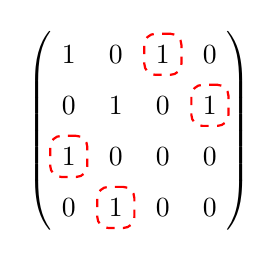
\begin{tikzpicture}[baseline=0cm]
    \matrix [mymatrix] (m)  
    {
    1 & 0 & 1 & 0 \\ 
    0 & 1 & 0 & 1 \\
    1 & 0 & 0 & 0 \\
    0 & 1 & 0 & 0 \\
    };

% parentheses
\coordinate (NW) at (m-1-1.north west);
\coordinate (SE) at (m-4-4.south east);

\node[xshift=4pt, fit=(NW)(SE), inner sep=0pt, left delimiter=(] {};
\node[xshift=-4pt, fit=(NW)(SE), inner sep=0pt, right delimiter=)] {};

\highlightcells[red]{1/3, 2/4, 3/1, 4/2}

\end{tikzpicture}
\end{center}

לכן,
\begin{align*}
\text{.} \det\prs{A} = \sgn\prs{\prs{3,4,1,2}} \cdot 1^4
\end{align*}
מתקיים
$\prs{3,4,1,2} = \prs{1;3} \prs{2;4}$
ולכן
\begin{align*}
\text{.} \det\prs{A} &= \sgn\prs{\prs{3,4,1,2}} = \prs{-1}^2 = 1
\end{align*}

\item במטריצה
$B$
אם נבחר את המקדם ה־%
$1$
בשורה הראשונה, נצטרך לבחור את המקדם ה־%
$4$
בשורה האחרונה (כי צריך להיות מקדם בעמודה ה־$4$, ואז את המקדם ה־%
$3$
בשורה השלישית (כי צריך להיות מקדם בעמודה ה־$3$), ואת המקדם ה־%
$2$
בשורה השנייה. כלומר, התמורה
$\sigma_1$
היחידה עבורה
$\sigma_1\prs{1} = 1$
שנצטרך להסתכל עליה בסכום היא
$\sigma_1 = \prs{1, 2, 3, 4} = \id_{[4]}$,
והגורם המתאים בחישוב הדטרמיננטה הוא
\[\text{.} \sgn\prs{\id_{[4]}} \prod_{i \in [4]} b_{i,i} = 1\]

\begin{center}
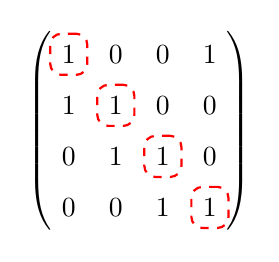
\begin{tikzpicture}[baseline=0cm]
    \matrix [mymatrix] (m)  
    {
    1 & 0 & 0 & 1 \\ 
    1 & 1 & 0 & 0 \\
    0 & 1 & 1 & 0 \\
    0 & 0 & 1 & 1 \\
    };

% parentheses
\coordinate (NW) at (m-1-1.north west);
\coordinate (SE) at (m-4-4.south east);

\node[xshift=4pt, fit=(NW)(SE), inner sep=0pt, left delimiter=(] {};
\node[xshift=-4pt, fit=(NW)(SE), inner sep=0pt, right delimiter=)] {};

\highlightcells[red]{1/1, 2/2, 3/3, 4/4}

\end{tikzpicture}
\end{center}

באופן דומה, אם בשורה הראשונה נבחר את המקדם ה־%
$1$,
נצטרך בשורה האחרונה לבחור את המקדם ה־%
$3$
ונקבל בסוף את בחירת המקדמים הבאה, המתאימה לתמורה
$\sigma_2 \coloneqq \prs{4, 1, 2, 3}$.

\begin{center}
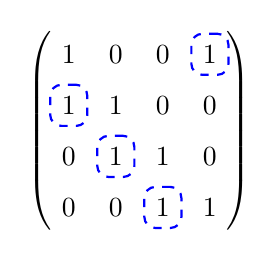
\begin{tikzpicture}[baseline=0cm]
    \matrix [mymatrix] (m)  
    {
    1 & 0 & 0 & 1 \\ 
    1 & 1 & 0 & 0 \\
    0 & 1 & 1 & 0 \\
    0 & 0 & 1 & 1 \\
    };

% parentheses
\coordinate (NW) at (m-1-1.north west);
\coordinate (SE) at (m-4-4.south east);

\node[xshift=4pt, fit=(NW)(SE), inner sep=0pt, left delimiter=(] {};
\node[xshift=-4pt, fit=(NW)(SE), inner sep=0pt, right delimiter=)] {};

\highlightcells[blue]{1/4, 2/1, 3/2, 4/3}

\end{tikzpicture}
\end{center}

ראינו בתרגיל קודם שסימן תמורה זאת הוא
$\sgn{\sigma_2} = \prs{-1}^{4-1} = -1$,
ולכן בסך הכל נקבל כי
\begin{align*}
\text{.} \det\prs{B} = \textcolor{red}{1} + \textcolor{blue}{\prs{-1}} = 0
\end{align*}

\item
נסמן
$n = m+k$.
לפי ההגדרה,
\begin{align*}
\text{.} \det\prs{C} = \sum_{\sigma \in S_n} \sgn\prs{\sigma} \prod_{i \in [n]} c_{i, \sigma\prs{i}}
\end{align*}
נשים לב כי אם
$\sigma\prs{i} = j$
עבור
$1 \leq i \leq m$
ועבור
$m+1 \leq j \leq m+k$,
המקדם
$c_{i,j}$
הוא מקדם של המטריצה
$0_{m \times k}$,
שהוא
$0$.
באופן דומה,
$c_{i,j} = 0$
כאשר
$m+1 \leq i \leq m+k$
וגם
$1 \leq j \leq m$.
לכן, כל תמורה שתורמת לסכום בדטרמיננטה היא הרכבה של תמורה על
$m$
האיברים הראשונים של
$[n]$
שמקבעת את שאר האיברים,
ותמורה של
$k$
האיברים שאחריהם שמקבעת את האיברים הראשונים.

נסמן
\begin{align*}
S &\coloneqq \set{\sigma \in S_n}{\forall i > m: \sigma\prs{i} = i} \\
S' &\coloneqq \set{\sigma \in S_n}{\forall i \leq m}{\sigma\prs{i} = i}
\end{align*}
ואז נקבל כי
\begin{align*}
\det\prs{C} &= \sum_{\substack{\sigma_1 \in S \\ \sigma_2 \in S'}} \sgn\prs{\sigma_1 \sigma_2} \prs{\prod_{i = 1}^m c_{i, \sigma_1\prs{i}}} \prs{\prod_{i = m+1}^{m+k} c_{i, \sigma_2\prs{i}}}
\\&=
\sum_{\substack{\sigma_1 \in S_m \\ \sigma_2 \in S_k}} \sgn\prs{\sigma_1}\sgn\prs{\sigma_2} \prs{\prod_{i = 1}^m x_{i, \sigma_1\prs{i}}} \prs{\prod_{i = 1}^{k} y_{i, \sigma_2\prs{i}}}
\\&=
\sum_{\sigma_1 \in S_m} \sgn\prs{\sigma_1} \prs{\prod_{i = 1}^m x_{i, \sigma_1\prs{i}}} \underbrace{\sum_{\sigma_2 \in S_k} \sgn\prs{\sigma_2} \prs{\prod_{i = 1}^{k} y_{i, \sigma_2\prs{i}}}}_{\det\prs{Y}}
\\&=
\det\prs{Y} \underbrace{\sum_{\sigma_1 \in S_m} \sgn\prs{\sigma_1} \prs{\prod_{i = 1}^m x_{i, \sigma_1\prs{i}}}}_{\det\prs{X}}
\\&=
\det\prs{Y} \det{X}
\\&= \det\prs{X} \det{Y}
\end{align*}
כנדרש.
\end{enumerate}
\end{solution}

\begin{remark}
שימו לב כי נובע באינדוקציה מהסעיף האחרון כי עבור מטריצה
\emph{אלכסונית בלוקים},
כלומר כזאת מהצורה
\[\pmat{
A_1 & 0 & \cdots & 0 & 0 \\
0 & A_2 & \ddots & \ddots & 0 \\
\vdots & \ddots & \ddots & \ddots & \vdots \\
0 & \ddots & \ddots & A_{n-1} & 0 \\
0 & 0 & \cdots & 0 & A_k
}\]
עבור
$A_i \in \Mat_{m_i}\prs{\FF}$
ועבור
$m_i \in \NN_+$,
מתקיים כי
\[\text{.} \det\prs{A} = \prod_{i \in [k]} \det\prs{A_i}\]
\end{remark}

\begin{exercisechap}
הראו לפי נוסחת הדטרמיננטה לפי תמורות כי הדטרמיננטה של מטריצה משולשת עליונה היא מכפלת איברי האלכסון.
\end{exercisechap}

\begin{solution}
תהי
$A \coloneqq \prs{a_{i,j}}_{i,j \in [n]} \in \Mat_n\prs{\FF}$
מטריצה משולשת עליונה. כלומר,
\[\text{.} \forall i > j: a_{i,j} = 0\]
אם
$\sigma \in S_n$
תמורה כך שיש
$i_0 \in [n]$
עם
$\sigma\prs{i_0} < i_0$,
נקבל כי
$a_{i_0, \sigma\prs{i_0}} = 0$
ולכן
$\prod_{i \in [n]} a_{i, \sigma\prs{i}} = 0$.
לכן, לפי הגדרת הדטרמיננטה,
$\det\prs{A}$
היא סכום הגורמים
$\sgn \sigma \prod_{i \in [n]} a_{i, \sigma\prs{i}}$
עבור התמורות
$\sigma$
עבורן
$\sigma\prs{i} \geq i$
לכל
$i \in [n]$.
אבל, תמורה היא חד־חד ערכית ועל, ולכן התמורה היחידה המקיימת זאת היא הזהות. לכן
\[det\prs{A} = \sgn\prs{\id_{[n]}} \prod_{i \in [n]} a_{i,i} = \prod_{i \in [n]} a_{i,i}\]
כנדרש.
\end{solution}

\begin{definition}[ערכים עצמיים ופולינום אופייני]
ניזכר מאלגברה א' כי
$\alpha \in \FF$
הינו
\emph{ערך עצמי}
של מטריצה
$A \in \Mat_n\prs{\FF}$
אם קיים
$v \in \FF^n$
עבורו
$Av = \alpha v$,
וכי הערכים העצמיים של
$A$
הם שורשי
\emph{הפולינום האופייני}
$p_A\prs{x} = \det\prs{x I - A}$.
\end{definition}

\begin{remark}
המטריצה
$xI - A$
אינה ב־%
$\Mat_n\prs{\FF}$,
כיוון ש־%
$x$
אינו איבר ב־%
$\FF$.

נחשב את הדטרמיננטה
$\det\prs{xI - A}$
באותו אופן שאנו מחשבות את הדטרמיננטה של מטריצה עם מקדמים בשדה
$\FF$.
\end{remark}

\begin{definition}[פולינום מתוקן]
פולינום
\[p\prs{x} = \sum_{i = 0}^n c_i x^i\]
נקרא
\emph{מתוקן}
אם עבור
$i \in \set{0, \ldots, n}$
המקסימלי כך ש־%
$c_i \neq 0$,
מתקיים כי
$c_i = 1$.
כלומר, אם המקדם של החזקה הגדולה ביותר שווה
$1$.
\end{definition}

בתרגיל הבא, ניעזר בדטרמיננטות כדי להראות שכל פולינום הינו פולינום אופייני של מטריצה.

\begin{exercisechap}
עבור פולינום מתוקן
$p \in \mbb{F}\brs{x}$
נכתוב
\[p\prs{x} = \sum_{i = 0}^n c_i x^i\]
כאשר
$c_n = 1$,
ונגדיר את
\emph{המטריצה המלווה של
$p$}
על ידי
\[\text{.} C\prs{p} \ceq \pmat{0 & 0 & \cdots & 0 & -c_0 \\ 1 & 0 & \cdots & 0 & -c_1 \\ 0 & 1 & \cdots & 0 & -c_2 \\ \vdots & \vdots & \ddots & \vdots & \vdots \\ 0 & 0 & \dots & 1 & -c_{n-1}} \in M_n\prs{\mbb{F}}\]

יהי
$p \in \mbb{F}\brs{x}$
ממעלה
$n$.
הראו כי הפולינום האופייני של
$C\prs{p}$
הוא
$p$.
\end{exercisechap}

\begin{solution}
מתקיים
\begin{align*}
\text{.} p_{C\prs{p}} &= \det\prs{I - xC\prs{p}}
= \det\pmat{x & 0 & \cdots & 0 & c_0 \\ -1 & x & \cdots & 0 & c_1 \\ 0 & -1 & \cdots & 0 & -c_2 \\ \vdots & \vdots & \ddots & \ddots & \vdots \\ 0 & 0 & \dots & -1 & x + c_{n-1}}
\end{align*}
ניעזר בכך שהטרמיננטה אינווריאנטית תחת הוספת כפולה של שורה לשורה אחרת.
נוסיף את השורה האחרונה כפול
$x$
לזאת שלפניה. לאחר מכן נוסיף את השורה ה־%
$n-1$
כפול
$x$
לזאת שלפניה ונמשיך כך עד שנקבל מטריצה
\begin{align*}
A \coloneqq \pmat{0 & 0 & \cdots & 0 & y \\ -1 & 0 & \cdots & 0 & * \\ 0 & -1 & \cdots & 0 & * \\ \vdots & \vdots & \ddots & \ddots & \vdots \\ 0 & 0 & \dots & -1 & *}
\end{align*}
כאשר
\[\text{.} y = a_0 + x\prs{a_1 + x\prs{a_2 + x\prs{\ldots \prs{a_{n-2} + x\prs{a_{n-1} + x}} \ldots}}} = \sum_{i=0}^n c_i x^i = p\]
נחשב כעת את הדטרמיננטה של
$A$
בעזרת תמורות. נשים לב כי לכל תמורה
$\sigma$
שאינה מקיימת
$\sigma\prs{1} = n$,
נקבל כי
$a_{1, \sigma\prs{1}} = 0$,
ולכן הגורם
$\sgn\prs{\sigma} \prod_{i = 0}^n a_{i, \sigma\prs{i}}$
יתאפס.
באותו אופן, לכל תמורה כזאת שאינה מקיימת
$\sigma\prs{i} = i-1$
לכל
$i \in \set{2, \ldots, n}$,
נקבל שהגורם המתאים לה בדטרמיננטה מתאפס, בגלל האפסים בשורות ה־%
$2, \ldots, n$.
לכן, אם נסמן
$\sigma \coloneqq \prs{n, 1, 2, \ldots, n-1}$
נקבל כי
\[\text{.} \det\prs{A} = \sgn\prs{\sigma} \cdot \prs{-1}^{n-1} p(x)\]
ראינו בתרגיל קודם כי
$\sgn\prs{\sigma} = \prs{-1}^{n-1}$
ולכן נקבל כי
\begin{align*}
\det\prs{C\prs{p}} = \det\prs{A} = \prs{-1}^{n-1} \prs{-1}^{n-1} p(x) = p(x)
\end{align*}
כנדרש.
\end{solution}

\section{כלל קרמר}

\subsection{מוטיבציה}

כלל קרמר מציג לנו דרך, בעזרת דטרמיננטות, לפתירה של מערכת משוואות לינארית
$Ax = b$.
תהי
$A \in \Mat_n\prs{\FF}$
הפיכה
ונסמן את העמודה ה־%
$i$
של
$A$
בתור
$v_i$.

כדי למצוא את המקדמים
$x_i$
של
$x$
ניזכר כי כפל של עמודה של
$A$
ב־%
$x_i$
כופל את הדטרמיננטה ב־%
$x_i$.
למשל, אם
$i=1, n=2$,
\begin{align}\label{eq:cramer-matrix}
\text{.} \det\pmat{\vert & \vert \\ x_1 v_1 & v_2 \\ \vert & \vert} = x_1 \det \pmat{\vert & \vert \\ v_1 & v_2 \\ \vert & \vert}
\end{align}
אם כן, נרצה לתאר את הדטרמיננטה שבאגף שמאל באופן אחר.

אבל, לפי הגדרת כפל מטריצות, מתקיים
$b = x_1 v_1 + x_2 v_2$
עבור
$\alpha_i \in \FF$
ונקבל כי
\begin{align*}
\det\pmat{\vert & \vert \\ b & v_2 \\ \vert & \vert} &=
\det\pmat{\vert & \vert \\ x_1 v_1 + x_2 v_2 & v_2 \\ \vert & \vert}
\\&=
x_1 \det\pmat{\vert & \vert \\ v_1 & v_2 \\ \vert & \vert}
+ x_2 \cancelto{0}{\det\prs{\pmat{\vert & \vert \\ v_2 & v_2 \\ \vert & \vert}}}
\\&=
x_1 \det\pmat{\vert & \vert \\ v_1 & v_2 \\ \vert & \vert}
\end{align*}
וזה בדיוק הביטוי שקיבלנו קודם ב־%
\eqref{eq:cramer-matrix}.
נקבל בסך הכל כי
\begin{align*}
\det\pmat{\vert & \vert \\ b & v_2 \\ \vert & \vert} = x_1 \det \pmat{\vert & \vert \\ v_1 & v_2 \\ \vert & \vert}
\end{align*}
ולכן
\begin{align*}
\text{.} x_1 = \frac{\det\pmat{\vert & \vert \\ b & v_2 \\ \vert & \vert}}{\det \pmat{\vert & \vert \\ v_1 & v_2 \\ \vert & \vert}}
\end{align*}
נקבל שוויון דומה עבור
$x_2$.

ראו איור
\ref{fig:cramer}
או עבור המחשה אינטרקטיבית, את
\href{https://colab.research.google.com/drive/1iqHCNg8T6HNnXnBdAzGhBw4rgD4fPG_L?usp=sharing#scrollTo=f9876309}{המחברת ב־\textenglish{Google Colab}}.

\begin{figure}[h]
\centering
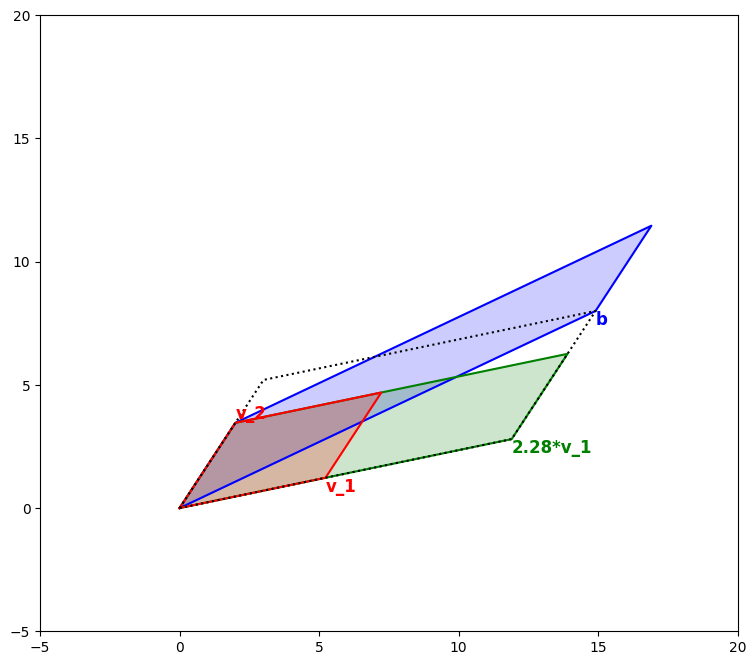
\includegraphics[width=0.5\textwidth]{images/cramer}
\caption{ויזואליזציה של כלל קרמר. שטח המקבילית הכחולה שווה $\det\prs{A_1}$, וזה שווה לשטח המקבילית הירוקה, השווה
$x_1 \det\prs{A}$.}
\label{fig:cramer}
\end{figure}

\begin{notation}
תהי
$A \in \Mat_n\prs{\FF}$
ויהי
$b \in \FF^n$.
עבור
$i \in [n]$,
נסמן ב־%
$A_i$
את המטריצה המתקבלת על ידי החלפת העמודה ה־%
$i$
של
$A$
ב־%
$b$.
\end{notation}

\begin{proposition}[כלל קרמר]
תהי
$A \in \Mat_n\prs{\FF}$
הפיכה
ויהי
$b \in \FF^n$.
למערכת המשוואות
\[Ax = b\]
קיים פתרון יחיד המתקבל על ידי
\begin{align*}
\text{.} \forall i \in [n]: x_i = \frac{\det\prs{A_i}}{\det\prs{A}}
\end{align*}
\end{proposition}

\subsection{תרגילים}

\begin{exercisechap}
תהי
\begin{align*}
T \colon \RR_2\brs{x} &\to \RR_2\brs{x} \\
p\prs{x} &\mapsto p\prs{x} + p\prs{x+1}
\end{align*}
ויהי
\[\text{.} q\prs{x} = x^2 + x + 1 \in \RR_2\brs{x}\]
מיצאו
$p \in \RR_2\brs{x}$
עבורו
$T\prs{p} = q$.
\end{exercisechap}

\begin{solution}
יהי
$\mcal{E} = \pmat{x^2, x, 1}$.
כיוון שההעתקה
\begin{align*}
\rho_\mcal{E} \colon \RR_2\brs{x} &\to \RR^3 \\
v &\mapsto \brs{v}_\mcal{E}
\end{align*}
הינה חד־חד ערכית, מתקיים
\[T\prs{p} = q\]
אם ורק אם
\[\text{.} \brs{T\prs{p}}_{\mcal{E}} = \brs{q}_\mcal{E}\]
ניזכר כי מתקיים תמיד
\[\brs{S\prs{v}}_{\mcal{B}} = \brs{S}_{\mcal{B}} \brs{v}_{\mcal{B}}\]
ולכן השוויון הנ"ל מתקיים בדיוק כאשר מתקיים השוויון
\[\text{.} \brs{T}_{\mcal{E}} \brs{p}_{\mcal{E}} = \brs{q}_{\mcal{E}}\]
כעת,
\begin{align*}
\brs{q}_\mcal{E} = \pmat{1 \\ 1 \\ 1}
\end{align*}
וכן
\begin{align*}
\brs{T}_{\mcal{E}} &= \pmat{\vert & \vert & \vert \\ \brs{T\prs{x^2}}_{\mcal{E}} & \brs{T\prs{x}}_{\mcal{E}} & \brs{T\prs{1}}_{\mcal{E}} \\ \vert & \vert & \vert}
\\&=
\pmat{\vert & \vert & \vert \\
\brs{2x^2 + 2x + 1}_{\mcal{E}} & \brs{2x + 1}_{\mcal{E}} & \brs{2}_{\mcal{E}} \\
\vert & \vert & \vert}
\\&=
\pmat{2 & 0 & 0 \\
2 & 2 & 0 \\
1 & 1 & 2}
\end{align*}
נסמן
\[A \coloneqq \pmat{2 & 0 & 0 \\
2 & 2 & 0 \\
1 & 1 & 2}\]
וגם
$b = \pmat{1 \\ 1 \\ 1}$
ואז מתקיים
$T\prs{p} = q$
אם ורק אם
$A \brs{p}_{\mcal{E}} = b$.
לפי כלל קרמר, זה מתקיים בדיוק כאשר
\begin{align*}
\text{.} \brs{p}_{\mcal{E}} &= \frac{1}{\det\prs{A}} \cdot \pmat{\det\prs{A_1} \\ \det\prs{A_2} \\ \det\prs{A_3}}
\end{align*}
כעת
\begin{align*}
\det\prs{A} &= \det \pmat{2 & 0 & 0 \\ 2 & 2 & 0 \\ 1 & 1 & 2} = 8 \\
\det\prs{A_1} &= \det\pmat{1 & 0 & 0 \\ 1 & 2 & 0 \\ 1 & 1 & 2} = 4 \\
\det\prs{A_2} &= \det\pmat{2 & 1 & 0 \\ 2 & 1 & 0 \\ 1 & 1 & 2} = 0 \\
\det\prs{A_3} &= \det\pmat{2 & 0 & 1 \\ 2 & 2 & 1 \\ 1 & 1 & 1} = 2 \det\pmat{2 & 1 \\ 1 & 1} + 1 \cancelto{0}{\det\pmat{2 & 2 \\ 1 & 1}}
\\&= 2 \prs{2 - 1}
\\&= 2
\end{align*}
כאשר שתי הדטרמיננטות הראשונות הן מכפלות איברי האלכסון כדטרמיננטות של מטריצות משולשות עליונות, והדטרמיננטה של
$A_2$
היא
$0$
כי יש שתי שורות שוות, ולכן השורות תלויות לינארית.

נקבל בסך הכל כי
\[ \brs{p}_{\mcal{E}} = \frac{1}{8} \pmat{4 \\ 0 \\ 2} = \pmat{1/2 \\ 0 \\ 1/4} \]
ולכן
\begin{align*}
\text{.} p\prs{x} = \frac{1}{2} \cdot x^2 + 0 \cdot x + \frac{1}{4} \cdot 1 = \frac{x^2}{2} + \frac{1}{4}
\end{align*}

נשים לב כי אכן
\begin{align*}
T\prs{p} &= p\prs{x} + p\prs{x+1} = \frac{x^2}{2} + \frac{1}{4} + \frac{\prs{x+1}^2}{2} + \frac{1}{4}
\\&= \frac{x^2}{2} + \frac{1}{2} + \frac{x^2 + 2x + 1}{2}
\\&= x^2 + x + 1
\\&= q\prs{x}
\end{align*}
כנדרש.
\end{solution}

\begin{exercisechap}
תהי
$A \in \Mat_n\prs{\RR}$
הפיכה עם מקדמים שלמים
ויהי
$b \in \RR^n$
וקטור עם מקדמים שלמים.
קבעו האם לפתרון המשוואה
$Ax = b$
יש מקדמים שלמים במקרים הבאים. הוכיחו או הפריכו את טענתכן.

\begin{enumerate}
\item $\det\prs{A} = 1$.
\item $\det\prs{A} = 2$.
\end{enumerate}
\end{exercisechap}

\begin{solution}
ראשית, ניזכר כי לפי כלל קרמר, פתרון המשוואה
$x$
מתקבל על ידי
\begin{align*}
\forall i \in [n]: x_i = \frac{\det\prs{A_i}}{\det\prs{A}}
\end{align*}
ונשים לב כי
$\det\prs{A_i} \in \ZZ$
כיוון שמקדמי
$A_i$
שלמים, והדטרמיננטה היא סכום של מכפלות של המקדמים. נעבור לדון בשני המקרים.

\begin{enumerate}
\item
במקרה בו
$\det\prs{A} = 1$,
נקבל כי
$x_i = \det\prs{A_i} \in \ZZ$
לכל
$i \in [n]$,
ולכן הוקטור
$x$
בעל מקדמים שלמים.

\item
במקרה בו
$\det\prs{A} = 2$,
אלא אם כל הדטרמיננטות
$\det\prs{A_i}$
מתחלקות ב־%
$2$,
לא כל מקדמי
$x$
יהיו שלמים. נמצא דוגמה נגדית.

תהי
$A = \pmat{1 & 1 \\ 2 & 4} \in \Mat_3\prs{\RR}$,
שמקדמיה אכן שלמים, ויהי
$b = \pmat{1 \\ 1} \in \RR^2$
שאכן מקדמיו שלמים.
נשים לב שגם אכן מתקיים
\begin{align*}
\text{.} \det\prs{A} = 1 \cdot 4 - 1 \cdot 2 = 4 - 2 = 2
\end{align*}

לפי כלל קרמר, פתרון
$Ax = b$
מתקבל על ידי
\begin{align*}
x_1 &= \frac{\det\pmat{1 & 1 \\ 1 & 4}}{\det\prs{A}} = \frac{4 - 1}{2} = \frac{3}{2} \notin \ZZ \\
x_2 &= \frac{\det\pmat{1 & 1 \\ 2 & 1}}{\det\prs{A}} = \frac{1 \cdot 1 - 1 \cdot 2}{2} = - \frac{1}{2} \notin \ZZ
\end{align*}
ולכן מקדמי
$x$
אינם כולם שלמים (ובעצם, אף אחד מהם אינו שלם).

יכולנו בעצם לבנות דוגמה בלי לנחש מקדמים. למשל, כדי למצוא
$A = \pmat{\vert & \vert \\ v_1 & v_2 \\ \vert & \vert} \in \Mat_2\prs{\RR}$
עבורה מקדמי הפתרון למערכת
$Ax = \pmat{1 \\ 1}$
אינם שלמים, נרצה
$x_1, x_2 \in \RR$
שאינם שלמים
עבורם
$x_1 v_1 + x_2 v_2 = \pmat{1 \\ 1}$.
נבחר למשל
$x_1 = x_2 = \frac{1}{2}$
ונקבל כי
$\frac{1}{2} \prs{v_1 + v_2} = \pmat{1 \\ 1}$
ואז
$v_1 + v_2 = \pmat{2 \\ 2}$.
נקבל כי אם
$A = \pmat{a & b \\ c & d}$,
מתקיים
\begin{align*}
2 &= \det\prs{A} = ad - bc \\
2 &= a + b \\
2 &= c + d
\end{align*}
ומכאן
\begin{align*}
b &= 2 - a \\
d &= 2 - c
\end{align*}
ואז
\begin{align*}
2 &= \det\prs{A}
\\&= a \prs{2-c} - \prs{2-a}c
\\&= 2a - ac - 2c + ac
\\&= 2a - 2c
\end{align*}
ולכן
$a-c = 1$.
נבחר למשל
$c = 1, a = 2$
ונקבל
$b = 2 - 2 = 0, d = 2 - 1 = 1$
כלומר
$A = \pmat{2 & 0 \\ 1 & 1}$
שמקדמיה אכן שלמים, והדטרמיננטה שלה אכן שווה
$2$
כמכפלת איברי האלכסון של מטריצה משולשת תחתונה.
אכן מתקיים
$A \pmat{1/2 \\ 1/2} = \pmat{1 \\ 1}$,
ולכן זאת דוגמה נגדית לסעיף.
\end{enumerate}
\end{solution}

\section{המטריצה המצורפת}

\subsection{מוטיבציה}

ניזכר כי כלל קרמר אומר שהפתרון של המערכת
$Ax = b$
עבור
$A \in \Mat_n\prs{\FF}$
הפיכה
ועבור
$b \in \FF^n$
מתקבל על ידי
\[\text{.} \forall i \in [n]: x_i = \frac{\det\prs{A_i}}{\det\prs{A}}\]
אם
$b = \pmat{b_1 \\ \vdots \\ b_n}$
עבור
$b_1, \ldots, b_n \in \FF$,
מתקיים לפי פיתוח דטרמיננטה לפי עמודה כי
\begin{align*}
\det\prs{A_i} &= \prs{-1}^{i+1} b_1 \det\prs{A_{\prs{1,i}}} + \ldots + \prs{-1}^{i+n} b_n \det\prs{A_{\prs{n,i}}}
\\&= \sum_{j \in [n]} \prs{-1}^{i+j} b_j \det\prs{A_{\prs{j,i}}}
\\&= \pmat{\prs{-1}^{i+1} \det\prs{A_{\prs{1,i}}} & \cdots & \prs{-1}^{i+n} \det\prs{A_{\prs{n,i}}}} b
\end{align*}
לכן אם נגדיר מטריצה
$\adj\prs{A} \in \Mat_n\prs{\FF}$
שמקיימת
$\prs{\adj\prs{A}}_{i,j} = \prs{-1}^{i+j} \det\prs{A_{\prs{j,i}}}$
לכל
$i,j \in [n]$,
נקבל כי
\[\adj\prs{A} b = \pmat{\det\prs{A_1} \\ \vdots \\ \det\prs{A_n}} = \det\prs{A} x\]
כאשר
$x$
הפתרון היחיד של המערכת
$Ax = b$.
נכתוב במקום זאת
$x = A^{-1} b$
ונקבל כי
$\adj\prs{A} b = \det\prs{A} A^{-1} b$.
כיוון שלא נעזרנו ב־%
$b$
בבניית
$\adj\prs{A}$,
המשוואה הזאת מתקיימת לכל
$b \in \FF^n$,
ולכן
$\adj\prs{A} = \det\prs{A} A^{-1}$.
אם נרצה לכתוב זאת אחרת, נכפול ב־%
$A$
מימין ונקבל
$\adj\prs{A} A = \det\prs{A}$.

\begin{definition}
תהי
$A \in \Mat_n\prs{\FF}$.
נגדיר
$\adj\prs{A} \in \Mat_n\prs{\FF}$
על ידי
\[\text{.} \forall i,j \in [n]: \prs{\adj\prs{A}}_{i,j} = \det\prs{A_{\prs{j,i}}}\]
\end{definition}

\begin{proposition}
לכל
$A \in \Mat_n\prs{\FF}$
הפיכה מתקיים
\[\adj\prs{A} = \det\prs{A} A^{-1}\]
ובאופן שקול
\[\text{.} \adj\prs{A} A = A \adj\prs{A} = \det\prs{A} I\]
\end{proposition}

\subsection{תרגילים}

\begin{exercisechap}
תהי
\begin{align*}
T \colon \Mat_2\prs{\CC} &\to \Mat_2\prs{\CC} \\
A &\mapsto i A + A^t
\end{align*}
מיצאו בעזרת המטריצה המצורפת את
$T^{-1}$.
\end{exercisechap}

\begin{solution}
יהי
$\mcal{E} = \prs{E_{1,1}, E_{1,2}, E_{2,1}, E_{2,2}}$
בסיס של
$V \coloneqq \Mat_2\prs{\CC}$
ונסמן
\begin{align*}
\text{.} A \coloneqq \brs{T}_{\mcal{E}} =
\pmat{
	1 + i & 0 & 0 & 0
	\\
	0 & i & 1 & 0
	\\
	0 & 1 & i & 0 \\
	0 & 0 & 0 & 1 + i
}
\end{align*}
אז לפי הטענה על המטריצה המשוכלפת מתקיים
\begin{align*}
\text{.} A^{-1} = \frac{\adj\prs{A}}{\det\prs{A}}
\end{align*}
נחשב את
$\adj\prs{A}, \det\prs{A}$
ונקבל מכך את
$A^{-1}$.
מתקיים
\begin{align*}
\det\prs{A} &= \prs{1+i}^2 \det\pmat{i & 1 \\ 1 & i}
\\&= \prs{1+i}^2 \prs{i^2 - 1^2}
\\&= \prs{1^2 + 2i + i^2} \prs{-2}
\\&= 2i \cdot \prs{-2}
\\ \text{.} \phantom{\det\prs{A}} &= -4i
\end{align*}
לכל
$j \neq 1$
מתקיים
$\det\prs{A_{\prs{1,j}}} = 0$
כי העמודה הראשונה של
$A_{\prs{1,j}}$
היא עמודת אפסים.
באותו אופן
$\det\prs{A_{\prs{i,1}}} = 0$
לכל
$i \neq 1$
כי אז השורה הראשונה במטריצה היא שורת אפסים.
מתקיים
\begin{align*}
\text{.} \det\prs{A_{1,1}} &= \det\pmat{i & 1 & 0 \\ 1 & i & 0 \\ 0 & 0 & 1+i}
\\&= \prs{i^2 - 1} \prs{1+i}
\\&= -2 - 2i
\end{align*}
באותו אופן,
$\det\prs{A_{\prs{4,j}}} = 0$
לכל
$j \neq 4$
וגם
$\det\prs{A_{\prs{i,4}}} = 0$
לכל
$i = 4$,
וכן
\begin{align*}
\text{.} \det\prs{A_{4,4}} &= \det\pmat{1+i & 0 & 0 \\ 0 & 1 & i \\ 0 & i & 1}
\\&= \prs{1+i} \prs{i^2 - 1}
\\&= -2 - 2i
\end{align*}
לכן
\begin{align*}
\adj\prs{A} &= \pmat{-2-2i & 0 & 0 \\ 0 & X & 0 \\ 0 & 0 & -2-2i}
\end{align*}
עבור מטריצה
$X \in \Mat_2\prs{\CC}$.

נחשב את שאר המקדמים.
\begin{align*}
\det\prs{A_{\prs{2,2}}} &= \det\pmat{1+i & 0 & 0 \\ 0 & i & 0 \\ 0 & 0 & 1+i}
\\&= \prs{1+i}^2 i \\&= 2i^2 \\&= -2 \\
\det\prs{A_{\prs{2,3}}} &= \det\pmat{1+i & 0 & 0 \\ 0 & 1 & 0 \\ 0 & 0 & 1+i}
\\&=
\prs{1+i}^2 \\&= 2i \\
\det\prs{A_{\prs{3,2}}} &= \det\pmat{1+i & 0 & 0 \\ 0 & 1 & 0 \\ 0 & 0 & 1+i}
\\&= \prs{1+i}^2
\\&= 2i \\
\det\prs{A_{\prs{3,3}}} &= \det\pmat{1+i & 0 & 0 \\ 0 & i & 0 \\ 0 & 0 & 1+i}
\\&=
\prs{1+i}^2 i
\\&= 2i \cdot i
\\&= -2
\end{align*}
לכן
\begin{align*}
\adj\prs{A} &= \pmat{
	-2-2i & 0 & 0 & 0 \\
	0 & -2 & -2i & 0 \\
	0 & -2i & -2 & 0 \\
	0 & 0 & 0 & -2-2i
}
\end{align*}
ולכן
\[\text{.} A^{-1} = \frac{1}{\det\prs{A}} \adj\prs{A} = \frac{1}{-4i} \pmat{
	-2-2i & 0 & 0 & 0 \\
	0 & -2 & -2i & 0 \\
	0 & -2i & -2 & 0 \\
	0 & 0 & 0 & -2-2i
}\]

אז, לכל
$a,b,c,d \in \CC$,
\begin{align*}
\text{.} T^{-1}\pmat{a & b \\ c & d} &= - \frac{1}{4i} \pmat{\prs{-2-2i}a & -2b - 2ic \\ - 2ib - 2c & \prs{-2-2i}d}
\end{align*}
ואז נוכל לשים לב שלכל
$X \in \Mat_2\prs{\CC}$
מתקיים
\[\text{.} T^{-1}\prs{X} = \frac{X + iX^t}{2i}\]
\end{solution}

\begin{exercisechap}
תהי
$A \in \Mat_n\prs{\RR}$
הפיכה עם מקדמים שלמים.
הוכיחו כי למטריצה
$A^{-1}$
מקדמים שלמים אם ורק אם
$\det\prs{A} \in \set{\pm 1}$.
מטריצה המקיימת זאת נקראת
\emph{אונימודולרית}.
\end{exercisechap}

\begin{solution}
\begin{itemize}
\item אם למטריצה
$A^{-1}$
מקדמים שלמים, מתקיים כי
$\det\prs{A}, \det\prs{A^{-1}} \in \ZZ$,
אבל אז
$\det\prs{A^{-1}} = \frac{1}{\det\prs{A}} \in \ZZ$
ולכן
$\det\prs{A}$
הינו מספר שלם שההופכי שלו גם הוא שלם, כלומר
$1$
או
$-1$.

\item נניח כי
$\det\prs{A} \in \set{\pm 1}$.
מתקיים
\begin{align*}
A^{-1} = \frac{1}{\det\prs{A}} \adj\prs{A}
\end{align*}
ולכן
\[\text{.} A^{-1} \in \set{\adj\prs{A}, -\adj\prs{A}}\]
אבל, מקדמי
$\adj\prs{A}$
הם סכומים של מכפלות של מקדמים של
$A$,
שהינם מספרים שלמים, ולכן גם מקדמי
$\adj\prs{A}$
שלמים, ואז גם מקדמי
$A^{-1}$.
\end{itemize}
\end{solution}

\begin{exercisechap}
הוכיחו או הפריכו את הטענה הבא.

אם
$A \in \Mat_n\prs{\FF}$
אלכסונית, גם
$\adj\prs{A}$
אלכסונית.
\end{exercisechap}

\begin{solution}
נסתכל על דוגמה לצורך כיוון. אם
$A = \pmat{1 & 0 & 0 \\ 0 & 2 & 0 \\ 0 & 0 & 3}$,
לכל אחת מבין
$A_{\prs{1,i}}$
עבור
$i \neq 1$
יש עמודת אפסים בתור העמודה הראשונה, ולכן
$\adj\prs{A}_{i,1} = 0$
לכל
$i \neq 1$.
באותו אופן,
$\adj\prs{A}_{1,j} = 0$
לכל
$j \neq 1$,
כיוון שהמקדם הוא דטרמיננטה של מטריצה שהשורה הראשונה שלה היא שורת אפסים.

נעבור למקרה הכללי. אם
$A$
אלכסונית, ו־%
$i,j \in [n]$
שונים, מתקיים כי
\[\text{.} \adj\prs{A}_{i,j} = \prs{-1}^{i+j} \det\prs{A_{\prs{i,j}}}\]
אם
$j > i$,
העמודה ה־%
$i$
של
$A_{\prs{i,j}}$
היא זאת של
$A$
בלי המקדם ה-%
$i,i$
(כיוון שחיסרנו מ־$A$ רק עמודה שלאחר העמודה ה־%
$i$).
אבל,
$A_{k,i} = 0$
לכל
$k \neq i$,
כיוון ש־%
$A$
אלכסונית, ולכן זאת עמודת אפסים.
אחרת,
$j < i$
ואז באותו אופן השורה ה־%
$j$
של
$A_{\prs{i,j}}$
היא שורת אפסים. בכל מקרה, נקבל כי
$\adj\prs{A}_{i,j} = 0$
לכל
$i,j \in [n]$
שונים, ולכן
$\adj\prs{A}$
אלכסונית.
\end{solution}

\section{הפולינום האופייני, ולכסינות}

\subsection{הגדרות ותכונות בסיסיות}

\begin{definition}[אופרטור לכסין]
אופרטור
$T \in \End\prs{V}$
נקרא
\emph{לכסין}
אם קיים בסיס
$\mcal{B}$
של
$V$
עבורו
$\brs{T}_{\mcal{B}}$
מטריצה אלכסונית.
\end{definition}

נתעניין באלגברה לינארית הרבה באופרטורים לכסינים. יתרון אחד של לכסינות, היא חישוב יעיל של חזקות. אם
$D = \diag\prs{\lambda_1, \ldots, \lambda_n}$
מטריצה לכסינה, ו־%
$\mcal{B}$
בסיס עבורו
$\brs{T}_{\mcal{B}} = D$,
נקבל כי לכל
$m \in \NN$
מתקיים
\[\brs{T^m}_{\mcal{B}} = D^n = \diag\prs{\lambda_1^m, \ldots, \lambda_n^m}\]
ולכן מצאנו בקלות מטריצה מייצגת של
$T^m$.

אם נכתוב
$\mcal{B} = \prs{v_1, \ldots, v_n}$
נשים לב מהגדרת מטריצה מייצגת שמתקיים
$T\prs{v_i} = \lambda_i v_i$.

\begin{definition}[ערכים ווקטורים עצמיים]
יהי
$T \in \End_\FF\prs{V}$
ויהי
$\lambda \in \FF$.
נגיד כי
$\lambda$
הינו
\emph{ערך עצמי של
$T$}
אם קיים
$v \in V \setminus \set{0}$
עבורו
$T\prs{v} = \lambda v$.
נקרא לוקטור
$v$
כזה
\emph{וקטור עצמי של
$T$
עבור הערך העצמי
$\lambda$}.
\end{definition}

נרצה לכמת ערכים עצמיים באופן שיגיד לנו, במקרה של אופרטורים לכסינים, כמה פעמים כל ערך מופיע על האלכסון. נשים לב כי עבור מטריצה לכסינה
$D = \diag\prs{\lambda_1, \ldots, \lambda_n}$,
מספר הפעמים ש־%
$\lambda$
מופיע על האלכסון, הוא הריבוי שלו כשורש של הפולינום
\[\text{.} p_D\prs{x} \coloneqq \det\prs{xI - D} = \prs{x - \lambda_1} \cdot \ldots \cdot \prs{x - \lambda_n}\]
לא כל פולינום יתפרק באופן כזה למכפלה של גורמים לינאריים, אבל נוכל תמיד להגדיר פולינום כזה.

\begin{definition}[פולינום אופייני]
תהי
$A \in \Mat_n\prs{\FF}$.
נגדיר את
\emph{הפולינום האופייני של
$A$}
בתור
\begin{align*}
\text{.} p_A\prs{x} = \det\prs{x I - A}
\end{align*}

נגדיר את
\emph{הפולינום האופייני}
של
$T \in \End_\FF\prs{V}$
בתור
$p_T\prs{x} = p_{\brs{T}_{\mcal{B}}}\prs{x}$
עבור
$\mcal{B}$
בסיס של
$V$.
\end{definition}

\begin{remark}
יתכן שבמהלך הקורס לא נציין כל הגדרה או טענה גם עבור אופרטורים וגם עבור מטריצות. הרבה מהטענות ניתן לתרגם בין אופרטורים ומטריצות באופן מיידי, וכאשר לא נציין את התרגום במפורש כדאי לנסות לחשוב עליו לבד.
\end{remark}

\begin{remark}
עבור
$T \in \End_\FF\prs{V}$
מתקיים
\[\text{.} p_T\prs{x} = \det\prs{x \id_V - T}\]
\end{remark}

\begin{proposition}
הערכים העצמיים של
$T \in \End_\FF\prs{V}$
הם שורשי הפולינום האופייני
$p_T\prs{x}$.
\end{proposition}

\begin{definition}[ריבוי אלגברי]
יהי
$T \in \End_\FF\prs{V}$
ויהי
$\lambda \in \FF$.
\emph{הריבוי האלגברי של
$\lambda$ ביחס ל־%
$T$}
הוא הריבוי של
$\lambda$
כשורש של
$p_T\prs{x}$.

נסמנו
$r_a^T\prs{\lambda}$,
או כאשר האופרטור ברור מההקשר, לעתים
$r_a\prs{\lambda}$.
\end{definition}

נוכל לחשב את מספר הפעמים שמופיע
$\lambda \in \FF$
על האלכסון של
המטריצה
$D \coloneqq \diag\prs{\lambda_1, \ldots, \lambda_n}$
באופן נוסף, בתור
$\dim \ker\prs{\lambda I - D}$,
כיוון שהמטריצה
$\lambda I - D$
היא מטריצה אלכסונית עם מספר אפסים על האלכסון השווה למספר הפעמים שמופיע
$\lambda$
על האלכסון של
$D$.

באופן כללי, הגרעין
$\ker\prs{\lambda \id_V - T}$
הוא אוסף כל הוקטורים העצמיים עם הערך העצמי
$\lambda$,
יחד עם וקטור האפס.

\begin{definition}[מרחב עצמי]
יהי
$T \in \End_\FF\prs{V}$
ויהי
$\lambda \in \FF$.
נסמן
\[V_\lambda^T \coloneqq \ker\prs{\lambda \id_V - T}\]
ונקרא לו
\emph{המרחב העצמי של
$T$
המתאים לערך העצמי
$\lambda$}.

כאשר האופרטור ברור מההקשר, נסמן לעתים
$V_\lambda$
עבור מרחב זה.
\end{definition}

\begin{definition}[ריבוי גיאומטרי]
יהי
$T \in \End_\FF\prs{V}$
ויהי
$\lambda \in \FF$.

\emph{הריבוי הגיאומטרי של
$\lambda$
כערך עצמי של
$T$}
הוא
\begin{align*}
\text{.} r^T_g\prs{\lambda} \coloneqq \dim V^T_{\lambda}
\end{align*}
כאשר האופרטור ברור מההקשר נסמן לעתים
$r_g\prs{\lambda}$
במקום זאת.
\end{definition}

\begin{proposition}
יהי
$T \in \End_\FF\prs{V}$
ויהי
$\lambda \in \FF$.
אז
\[\text{.} r_g^T\prs{\lambda} \leq r_a^T\prs{\lambda}\]
\end{proposition}

\begin{proposition} \label{proposition:diag-equivalence}
יהי
$T \in \End_\FF\prs{V}$.
התנאים הבאים שקולים.

\begin{enumerate}[label = (\alph*)]
\item $T$ לכסין.
\item הפולינום
$p_T\prs{x}$
מתפצל כמכפלה של גורמים לינאריים, ולכל ערך עצמי
$\lambda \in \FF$
מתקיים
$r_a\prs{\lambda} = r_g\prs{\lambda}$.
\item אם הערכים העצמיים השונים של
$T$
הם
$\lambda_1, \ldots, \lambda_k$
ואם
$\mcal{B}_1, \ldots, \mcal{B}_k$
בסיסים של
$V_{\lambda_1}, \ldots, V_{\lambda_k}$
בהתאמה, אז
\[\mcal{B} \coloneqq \bigcup_{i \in [k]} \mcal{B}_i\]
הוא בסיס של
$V$.
\end{enumerate}
\end{proposition}

\subsection{תרגילים}

\begin{exercisechap}
הוכיחו כי המטריצה
\[A = \pmat{a & b \\ 0 & c} \in \Mat_2\prs{\RR}\]
הינה לכסינה אם ורק אם
$b = 0$
או
$a \neq c$.
\end{exercisechap}

\begin{solution}
ניזכר ראשית שהערכים העצמיים של מטריצה משולשת עליונה הינם איברי האלכסון, וכי הריבוי האלגברי של כל ערך עצמי הוא מספר הפעמים שהוא מופיע על האלכסון. לכן הערכים העצמיים של
$A$
הם
$a,c$
כאשר אם
$a = c$,
זהו ערך עצמי מריבוי אלגברי
$2$
ואחרת כל אחד מריבוי אלגברי
$1$.

נניח כעת כי
$A$
לכסינה וכי
$a=c$,
ונראה כי
$b \neq 0$.

$a$
ערך עצמי מריבוי אלגברי
$2$.
הריבוי האלגברי של ערך עצמי במטריצה לכסינה הוא מספר הפעמים שהוא מופיע על האלכסון במטריצה אלכסונית הדומה לה, ולכן
$A$
דומה ל־%
$a I$.
אבל, המטריצה היחידה הדומה ל־%
$a I$
היא עצמה, כיוון שלכל
$P \in \Mat_2\prs{\RR}$
הפיכה מתקיים
\[\text{.} P^{-1} a I P = a P^{-1} I P = a P^{-1} P = a I\]
לכן
$A = aI$
ולכן
$b = 0$.

נניח בכיוון השני כי
$a \neq c$
או
$b = 0$,
ונוכיח כי
$A$
לכסינה.

אם
$b = 0$,
המטריצה
$A$
אלכסונית בעצמה, ואין מה להראות. נניח אם כן כי
$a \neq c$.
אז
\begin{align*}
p_A\prs{x} &= \det\pmat{x - a & -b \\ 0 & x - c}
\\&= \prs{x-a}\prs{x-c}
\end{align*}
מתפצל לגורמים לינאריים ובנוסף
\begin{align*}
1 \leq r_g\prs{a} \leq r_a\prs{a} = 1 \\
1 \leq r_g\prs{c} \leq r_a\prs{c} = 1
\end{align*}
ולכן
$r_g\prs{a} = r_a\prs{a} = 1$
וכן
$r_g\prs{c} = r_a\prs{c} = 1$.
לכן מטענה
\ref{proposition:diag-equivalence}
המטריצה
$A$
לכסינה.
\end{solution}

\begin{exercisechap}
נסתכל על מטריצת הסיבוב הבאה, התלויה בפרמטר
$\theta \in \RR$.

\begin{align*}
\text{.} \rho_\theta \coloneqq \pmat{\cos\prs{\theta} & -\sin\prs{\theta} \\ \sin\prs{\theta} & \cos\prs{\theta}} \in \Mat_2\prs{\RR}
\end{align*}

\begin{enumerate}
\item קיבעו עבור אילו ערכי
$\theta$
המטריצה
$\rho_\theta$
לכסינה. עבור הערכים שעבורם היא לכסינה, מיצאו מטריצה
$2 \times 2$
הפיכה
$P$
ומטריצה אלכסונית
$D$
עבורן
\[\text{.} P^{-1} \rho_\theta P = D\]

\item איך תשתנה תשובתכן לסעיף הקודם אם נסתכל על
$\rho_\theta$
כעל מטריצה ב־%
$\Mat_2\prs{\CC}$?
\end{enumerate}
\end{exercisechap}

\begin{solution}
\begin{enumerate}
\item
נחשב ערכים עצמיים, שהם שורשי הפולינום האופייני.
\begin{align*}
p_{\rho_\theta}\prs{x} &= \det\prs{xI - \rho_\theta}
\\&= \det\pmat{x - \cos\prs{\theta} & \sin\prs{\theta} \\
- \sin\prs{\theta} & x - \cos\prs{\theta}}
\\&=
\prs{x-\cos\prs{\theta}}^2 + \sin\prs{\theta}^2
\\&= x^2 - 2 \cos\prs{\theta} x + \cos\prs{\theta}^2 \sin\prs{\theta}^2
\\&= x^2 - 2 \cos\prs{\theta} x + 1
\end{align*}
שורשי הפולינום, לפי נוסחת השורשים של פולינום ריבועי, הם
\begin{align*}
x_{1,2} &\coloneqq \frac{2 \cos\prs{\theta} \pm \sqrt{\prs{2\cos\prs{\theta}}^2 - 4}}{2}
\\&=
\frac{2 \cos\prs{\theta} \pm 2 \sqrt{\cos\prs{\theta}^2 - 1}}{2}
\\&=
\cos\prs{\theta} \pm \sqrt{- \sin\prs{\theta}^2}
\\&=
\cos\prs{\theta} \pm i \sin\prs{\theta}
\end{align*}
ונסמן
\begin{align*}
x_1 &= \cos\prs{\theta} + i \sin\prs{\theta} \\
\text{.} x_2 &= \cos\prs{\theta} - i \sin\prs{\theta}
\end{align*}

אם
$\sin\prs{\theta} \neq 0$
נקבל כי אין ערכים עצמיים ממשיים. לכן אין שורשים ממשיים לפולינום
$p_{\rho_\theta}$,
לכן הוא אינו מתפצל כמכפלה של גורמים לינאריים, ולכן לפי טענה
\ref{proposition:diag-equivalence}
המטריצה
$\rho_\theta$
אינה לכסינה.

אחרת,
$\sin\prs{\theta} = 0$
ואז
\begin{align*}
\rho_\theta = \pmat{\cos\prs{\theta} & 0 \\ 0 & \cos\prs{\theta}}
\end{align*}
והמטריצה לכסינה כמטריצה אלכסונית. נבחר למשל
$P = I$
ונקבל כי
\[D \coloneqq P^{-1} \rho_\theta P = \rho_\theta = \pmat{\cos\prs{\theta} & 0 \\ 0 & \cos\prs{\theta}}\]
אלכסונית.

\item כאשר
$\sin\prs{\theta} = 0$,
המטריצה
$\rho_\theta$
עדיין לכסינה באותו אופן.

כאשר
$\sin\prs{\theta} \neq 0$,
נקבל הפעם שני ערכים עצמיים
$\cos\prs{\theta} \pm i \sin\prs{\theta}$
שונים, כל אחד מריבוי אלגברי
$1$.
כיוון שהריבוי הגיאומטרי של ערך עצמי שווה לפחות
$1$
ואינו גדול מהריבוי האלגברי, נקבל כי הריבויים הגיאומטריים של הערכים העצמיים גם הם שווים
$1$.
נמצא וקטורים עצמיים.

\begin{itemize}
\item עבור הערך העצמי
$x_1 = \cos\prs{\theta} + i \sin\prs{\theta}$,
הוקטורים העצמיים הם הוקטורים בגרעין של
\[\text{.} x_1 I - \rho_\theta = \pmat{x_1 - \cos\prs{\theta} & \sin\prs{\theta} \\ -\sin\prs{\theta} & x_1 - \cos\prs{\theta}} = \pmat{i \sin\prs{\theta} & \sin\prs{\theta} \\ -\sin\prs{\theta} & i \sin\prs{\theta}}\]
זאת מטריצה שהעמודה הראשונה שלה שווה לעמודה השנייה כפול
$i$,
ולכן דרגתה
$1$,
והוקטור
$\pmat{1 \\ -i}$
הינו וקטור עצמי שלה עם ערך עצמי
$0$,
ולכן וקטור עצמי של
$\rho_\theta$
עם ערך עצמי
$x_1$.
הראנו כי הריבוי הגיאומטרי שווה
$1$,
ולכן וקטור עצמי זה פורש את כל המרחב העצמי (שהינו ממימד $1$)
ונקבל כי
\begin{align*}
\text{.} V^{\rho_\theta}_{x_1} = \Span\prs{\pmat{1 \\ -i}}
\end{align*}

\item עבור הערך העצמי
$x_2 = \cos\prs{\theta} - i \sin\prs{\theta}$,
הוקטורים העצמיים הם הוקטורים בגרעין של
\begin{align*}
\text{.} x_2 I - \rho_\theta = \pmat{-i\sin\prs{\theta} & \sin\prs{\theta} \\ -\sin\prs{\theta} & -i \sin\prs{\theta}}
\end{align*}
זאת מטריצה שהעמודה הראשונה שללה שווה לעמודה השנייה כפול
$-i$
ולכן דרגתה
$1$
והוקטור
$\pmat{1 \\ i}$
הוא וקטור עצמי שלה עם ערך עצמי
$0$
ובאותו אופן כמו עם הערך העצמי הקודם,
\[\text{.} V_{x_2}^{\rho_\theta} = \Span\prs{\pmat{1 \\ i}}\]
\end{itemize}
נקבל בסך הכל כי
$\mcal{B} \coloneqq \prs{\pmat{1 \\ -i}, \pmat{i \\ i}}$
בסיס של
$V$
המורכב מוקטורים עצמיים של
$\rho_\theta$.
אז
\[D \coloneqq \brs{T_{\rho_\theta}}_{\mcal{B}} = \diag\prs{x_1, x_2}\]
ומתקיים
\begin{align*}
D = \prs{M^{\mcal{B}}_{\mcal{E}}}^{-1} \brs{T_{\rho_\theta}}_{\mcal{E}} M^{\mcal{B}}_{\mcal{E}}
\end{align*}
לפי נוסחת מעבר בסיס. לכן אם נסמן
\begin{align*}
P \coloneqq M^{\mcal{B}}_{\mcal{E}} = \pmat{1 & 1 \\ -i & i}
\end{align*}
נקבל כי
\begin{align*}
D = P^{-1} \rho_B P
\end{align*}
מטריצה אלכסונית.
\end{enumerate}
\end{solution}

\begin{exercisechap}
תהי
\begin{align*}
\text{.} A = \pmat{-3 & -4 & -6 & -3 & -3 & 0 \\ -2 & -3 & -4 & -3 & -3 & 0 \\ 3 & 3 & 5 & 3 & 3 & 0 \\ -1 & 2 & 1 & 2 & 0 & 0 \\ 2 & 1 & 3 & 0 & 2 & 0 \\ 3 & 3 & 3 & 3 & 3 & 2} \in \Mat_6\prs{\mbb{C}}
\end{align*}

מיצאו את הערכים העצמיים של
$A$
ועבור כל אחד מהם מיצאו ריבוי אלגברי וגיאומטרי.
\end{exercisechap}

\begin{solution}
נחשב ראשית את הפולינום האופייני של
$A$.

\begin{align*}
p_A\prs{x} &= \det\prs{xI - A}
\\&=
\det\pmat{x +3 & 4 & 6 & 3 & 3 & 0 \\
2 & x+3 & 4 & 3 & 3 & 0 \\
-3 & -3 & x-5 & -3 & -3 & 0 \\
1 & -2 & -1 & x-2 & 0 & 0 \\
-2 & -1 & -3 & 0 & x-2 & 0 \\
-3 & -3 & -3 & -3 & -3 & x-2}
\\&=
\prs{x-2} \pmat{x +3 & 4 & 6 & 3 & 3 \\
2 & x+3 & 4 & 3 & 3 \\
-3 & -3 & x-5 & -3 & -3 \\
1 & -2 & -1 & x-2 & 0\\
-2 & -1 & -3 & 0 & x-2}
\\&= \ldots
\\ \text{.} \hphantom{p_A\prs{x}} &= \prs{x-2} \prs{x^5 - 3x^4 + x^3 + x^2 + 4}
\end{align*}
ניתן לראות כי
$2$
הינו ערך עצמי של
$A$,
כי הוא שורש של
$p_A\prs{x}$.
נחשב את הריבוי שלו
$r_a\prs{2}$,
ששווה לערך
$i \in \mbb{N}$
המינימלי עבורו
$p_A\prs{x}^{\prs{i}}\prs{2} \neq 0$,
כאשר
$f^{\prs{k}}$
הינה הנגזרת ה־%
$k$-ית
של
$f$.
מתקיים
\begin{align*}
p_A\prs{x} &= x^6 - 5x^5 + 7x^4 - x^3 -2x^2 + 4x - 8
\\
p_A'\prs{x} &= 6x^5 - 25x^4 + 28x^3 - 3x^2 -4x + 4
\\
p_A'\prs{2} &= 6 \cdot 32 - 20 \cdot 16 + 28 \cdot 8 - 3 \cdot 4 - 4 \cdot 2 + 4 = 0
\\
p_A''\prs{x} &= 30x^4 - 100x^3 + 84 x^2 - 6x - 4
\\
p_A''\prs{2} &= 30\cdot 16 - 100\cdot 8 + 84 \cdot 4 - 6 \cdot 2 - 4 = 0
\\
p_A'''\prs{x} &= 120 x^3 - 300 x^2 + 168 x - 6
\\
p_A'''\prs{2} &= 120 \cdot 8 - 300 \cdot 4 + 168 \cdot 2 - 6 = 90 \neq 0
\end{align*}
ולכן
$r_a\prs{2} = 3$.
נקבל כי
$\prs{x-2}^3 = x^3 - 6x^2 + 12x - 8$
מחלק את
$p_A\prs{x}$
וכדי למצוא ערכים עצמיים נוספים נבצע חילוק פולינומים.

בכל שלב נכפול את הפולינום בו אנו מחלקות במונום מתאים כך שהכפל יהיה בעל אותו גורם מוביל כמו הפולינום שקיבלנו לאחר חיסור בשלב הקודם, ולאחר מכן נחסר זאת מהפולינום שקיבלנו בשלב הקודם. נסכום את המונומים המתאימים כדי לקבל את המנה, כאשר אם נשארנו עם פולינום מדרגה קטנה יותר מזה שאנו מחלקות בו, הוא יהיה שארית החלוקה.

\begin{center}
\polylongdiv{x^6-5x^5+7x^4-x^3-2x^2+4x-8}{x^3-6x^2+12x-8}
\end{center}

לכן
\[p_A\prs{x} = \prs{x-2}^3 \prs{x^3 + x^2 + x + 1}\]
וניתן לראות כי
$-1$
שורש של
$x^3 + x^2 + x + 1$
(הוא שורש של כל פולינום ממעלה אי־זוגית שכל מקדמיו
$1$)ץ
נבצע חילוק פולינומים נוסף

\begin{center}
\polylongdiv{x^3+x^2+x+1}{x+1}
\end{center}

ולכן
\[p_A\prs{x} = \prs{x-2}^3 \prs{x+1} \prs{x^2 + 1} = \prs{x-2}^3 \prs{x+1} \prs{x + i} \prs{x - i}\]
ונקבל כי הערכים העצמיים הם
$2$
מריבוי אלגברי
$3$,
ו־%
$-1, i, -i$
כל אחד מריבוי אלגברי
$1$.

כיוון שהריבוי הגיאומטרי תמיד גדול או שווה ל־%
$1$
וקטן או שווה לריבוי האלגברי, נקבל כי
$r_g\prs{-1} = r_g\prs{i} = r_g\prs{-i} = 1$
ולכן נותר למצוא את הריבוי הגיאומטרי של
$2$,
ששווה לדרגת המטריצה
$A - 2I$.
נחשב דרגה זאת.

\begin{align*}
A - 2I &=
\pmat{-5 & -4 & -6 & -3 & -3 & 0 \\
-2 & -5 & -4 & -3 & -3 & 0 \\
3 & 3 & 3 & 3 & 3 & 0 \\
-1 & 2 & 1 & 0 & 0 & 0 \\
2 & 1 & 3 & 0 & 0 & 0 \\
3 & 3 & 3 & 3 & 3 & 0}
\\& \xrightarrow{C_5 \mapsto C_5 - C_4}
\pmat{-5 & -4 & -6 & -3 & 0 & 0 \\
-2 & -5 & -4 & -3 & 0 & 0 \\
3 & 3 & 3 & 3 & 0 & 0 \\
-1 & 2 & 1 & 0 & 0 & 0 \\
2 & 1 & 3 & 0 & 0 & 0 \\
3 & 3 & 3 & 3 & 0 & 0}
\\& \xrightarrow{\substack{C_1 \mapsto C_1 - C_4 \\ C_2 \mapsto C_2 - C_4 \\ C_3 \mapsto C_3 - C_4}}
\pmat{-2 & -1 & -3 & -3 & 0 & 0 \\
1 & -2 & -1 & -3 & 0 & 0 \\
0 & 0 & 0 & 3 & 0 & 0 \\
-1 & 2 & 1 & 0 & 0 & 0 \\
2 & 1 & 3 & 0 & 0 & 0 \\
0 & 0 & 0 & 3 & 0 & 0}
\\& \xrightarrow{C_3 \mapsto C_3 - C_1 - C_2}
\pmat{-2 & -1 & 0 & -3 & 0 & 0 \\
1 & -2 & 0 & -3 & 0 & 0 \\
0 & 0 & 0 & 3 & 0 & 0 \\
-1 & 2 & 0 & 0 & 0 & 0 \\
2 & 1 & 0 & 0 & 0 & 0 \\
0 & 0 & 0 & 3 & 0 & 0}
\end{align*}
וניתן לראות מכאן כי
$\rank\prs{A-2I} = 3$,
לכן
$r_g\prs{2} = 3$.

\end{solution}

\begin{exercisechap}
\begin{enumerate}
\item תהיינה
$A,B \in \Mat_n\prs{\FF}$
ונניח כי
$B$
לכסינה ועם
$n$
ערכים עצמיים שונים
$\lambda_1, \ldots, \lambda_n$,
וכי
$AB = BA$.

הוכיחו כי
$A$
לכסינה.

\item הוכיחו כי
\begin{align*}
B = \pmat{0 & 1 & 0 & \cdots & 0 \\ 0 & 0 & 1 & \ddots & \vdots \\ \vdots & \ddots & \ddots & \ddots & 0 \\ 0 & \ddots & \ddots & 0 & 1 \\ 1 & 0 & \cdots & \cdots & 0} \in \Mat_n\prs{\CC}
\end{align*}
הינה לכסינה, מיצאו
$P \in \Mat_n\prs{\CC}$
עבורה
$P^{-1} B P$
אלכסונית,
והראו כי כל מטריצה
$A \in \Mat_n\prs{\CC}$
עבורה
$AB = BA$
גם היא לכסינה.
\end{enumerate}
\end{exercisechap}

\begin{solution}
\begin{enumerate}
\item
נרצה להשתמש בהגדרה של ערכים עצמיים, ולכן נרצה וקטורים עצמיים מתאימים.
יהי
$\mcal{B} \coloneqq \prs{v_1, \ldots, v_n}$
בסיס של
$\FF^מ$
עבורו
$B v_i = \lambda_i$
לכל
$i \in [n]$.

אז, לכל
$i \in [n]$,
\begin{align*}
\text{.} BA v_i = AB v_i = \lambda_i A v_i
\end{align*}
אם
$A v_i = 0$
נקבל כי
$v_i$
וקטור עצמי של
$A$
עם ערך עצמי
$0$,
ואחרת נקבל כי
$A v_i$
וקטור עצמי של
$B$
עם ערך עצמי
$\lambda_i$,
אך כיוון ש־%
$V^B_{\lambda_i} = \Span\prs{v_i}$
נקבל כי
$A v_i \in \Span\prs{v_i}$.
כלומר, קיים
$\mu_i \in \FF$
עבורו
$A v_i = \mu_i v_i$,
ולכן
$v_i$
וקטור עצמי של
$A$
עם ערך עצמי
$\mu_i$.
נקבל בסך הכל כי כל
$v_i$
הוא וקטור עצמי של
$A$,
ולכן
$\mcal{B}$
בסיס מלכסן גם של
$A$.

\item
נחפש את הערכים העצמיים האפשריים של
$B$.
יהי
$\lambda \in \CC$
ערך עצמי. אז קיים
\begin{align*}
v = \pmat{v_1 \\ \vdots \\ v_{n-1}} \in \CC^n
\end{align*}
עבורו
\begin{align*}
\lambda v = Bv = \pmat{v_2 \\ v_3 \\ \vdots \\ v_n \\ v_1}
\end{align*}
ולאחר כפל משמאל
$n$
פעמים ב־%
$B$
נקבל
\begin{align*}
\text{.} \lambda^n v = B^n v = v
\end{align*}
לכן
$\lambda^n = 1$
ולכן
\[\text{.} \lambda \in \set{\mathrm{cis}\prs{\frac{2 \pi k}{n}}}{k \in [n]}\]
נראה שאכן כל ערך בקבוצה זאת הוא ערך עצמי, ונקבל
$n$
ערכים עצמיים שונים. אכן הערך
\[\lambda_k \coloneqq \mathrm{cis}\prs{\frac{2 \pi k}{n}}\]
הוא ערך עצמי עם וקטור עצמי
\[u_k \coloneqq \pmat{1 \\ \lambda_k \\ \vdots \\ \lambda_k^{n-1}}\]
שכן
\begin{align*}
\text{.} A u_k = \pmat{\lambda_k \\ \vdots \\ \lambda_k^{n-1} \\ 1} = \lambda_k \pmat{1 \\ \lambda_k \\ \vdots \\ \lambda_k^{n-1}} = \lambda_k u_k
\end{align*}

כעת, כדי למצוא
$P \in \Mat_n\prs{\CC}$
עבורה
$P^{-1} B P$
אלכסונית, ניקח מטריצה שעמודותיה הן איברי הבסיס
$\mcal{B} \coloneqq \prs{u_1, \ldots, u_n}$.
כדי לראות זאת, נשים לב כי
\begin{align*}
\brs{T_B}_{\mcal{B}} = \diag\prs{\lambda_1, \ldots, \lambda_n}
\end{align*}
ונקבל לפי נוסחאת מעבר בסיס כי
\begin{align*}
\diag\prs{\lambda_1, \ldots, \lambda_n} &= \brs{T_B}_{\mcal{B}}
\\
\\&=
\prs{M^{\mcal{B}}_{\mcal{E}}}^{-1} \brs{T_B}_{\mcal{E}} M^{\mcal{B}}_{\mcal{E}}
\end{align*}
ולאחר סימון
\begin{align*}
P \coloneqq M^{\mcal{B}}_{\mcal{E}}
\end{align*}
נקבל כי
\begin{align*}
P^{-1} B P = \diag\prs{\lambda_1, \ldots, \lambda_n}
\end{align*}
אלכסונית, כנדרש.

לבסוף, נציין שכיוון ש־%
$B$
לכסינה עם
$n$
ערכים עצמיים שונים, לפי הסעיף הראשון כל מטריצה
$A \in \Mat_n\prs{\CC}$
המתחלפת איתה גם היא לכסינה.

לפי דרך הפתרון של הסעיף הראשון נראה אפילו כי
$P^{-1} A P$
אלכסונית לכל
$A$
כזאת.
\end{enumerate}
\end{solution}

\begin{remark}
מטריצות המתחלפות עם המטריצה
$B$
מהסעיף הקודם נקראות
\emph{סירקולנטיות}
\textenglish{(circulant)}
ויש להן שימושים באנליזה נומרית וקריפטוגרפיה.
\end{remark}

\printbibliography
\end{document}
